\documentclass[12pt,a4paper]{article}

\usepackage[english]{babel}
\usepackage[utf8]{inputenc}
\usepackage{amsmath}
\usepackage{amsfonts}
\usepackage{amssymb}
\usepackage{float}
\usepackage{graphicx}
\usepackage{enumitem}
% \usepackage[colorinlistoftodos]{todonotes}
\usepackage[margin=0.8in]{geometry}
% \usepackage{wrapfig}
\usepackage[justification=centering]{caption}
\usepackage[subnum]{cases}
\setlength{\parindent}{0pt}
\setlength{\parskip}{1em}
\usepackage{empheq}
\usepackage{mlmodern}
\usepackage{amsthm}
\usepackage{listings}
\usepackage{hyperref}
\usepackage{xcolor} % Predefines additional colors and allows user defined colors
% code styling
\definecolor{codegreen}{rgb}{0,0.6,0}
\definecolor{codegray}{rgb}{0.5,0.5,0.5}
\definecolor{codepurple}{rgb}{0.58,0,0.82}
\definecolor{backcolour}{rgb}{1,1,1}
\lstdefinestyle{mystyle}{
    backgroundcolor=\color{backcolour},   
    commentstyle=\color{codegreen},
    keywordstyle=\color{magenta},
    frame=single,
    numberstyle=\tiny\color{codegray},
    stringstyle=\color{codepurple},
    basicstyle=\ttfamily\footnotesize,
    breakatwhitespace=false,         
    breaklines=true,                 
    captionpos=b,                    
    keepspaces=true,                 
    numbersep=5pt,                  
    showspaces=false,                
    showstringspaces=false,
    showtabs=false,                  
    tabsize=2
}
\lstset{style=mystyle}

\title{\textsc{\large Numerical Assignment\\Condensed Matter Physics} \\ {\bf Nearly Free Electron Model}}
\author{Gayatri P\\Int. M.Sc. (3rd Year)\\ (2211185)}

\begin{document}
\maketitle
\newcommand{\cfunc}[1]{\textnormal{\texttt{\detokenize{#1}}}}
\tableofcontents
\section{Theory}
\subsection{Introduction}
We start with completely free electrons whose Hamiltonian is
\begin{align*}
    H_0 = \frac{q^2}{2m}
\end{align*}
For a free electron, this leads to the free electron band structure in the $q$ basis which is given by Schrodinger's equation
\begin{align*}
    \left[\frac{(\hbar q + \hat{p})^2}{2m}\right]\psi_q = E_q\psi_q
\end{align*} 

\begin{figure}[H]
    \centering
    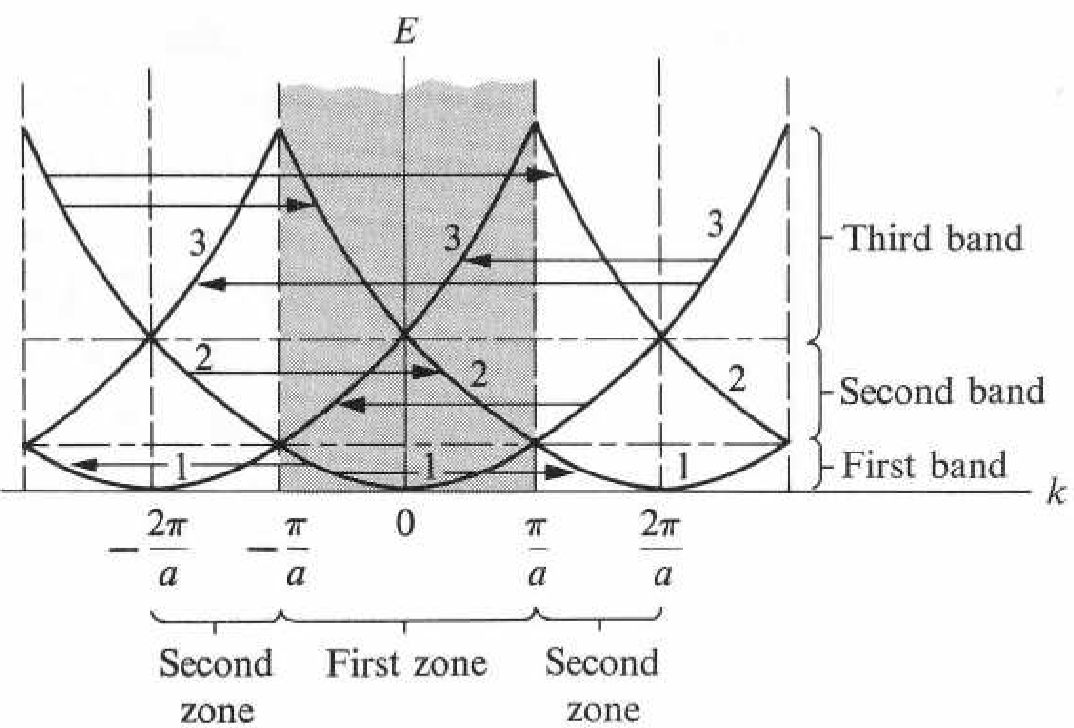
\includegraphics[width=0.7\linewidth]{images/th1.png}
    \caption{Free Electron Band Structure. The shaded region is the Brillouin Zone.}
\end{figure}

Now consider a weak periodic potential perturbation to this Hamiltonian,
\begin{align*}
    H = H_0 + V(x)
\end{align*}
where $V$ is periodic in the lattice space.
\begin{align*}
    V(x+la) = V(x)
\end{align*}
Due to its periodicity, one can also chose to expand $V$ in the fourier space as
\begin{align*}
    V= \sum_{G} V_G e^{iGx}
\end{align*}
where $G=2\pi x/a$. We will now see mathematically, how this changes the energy band structure of the electron.

\subsection{Mathematical Description} \label{1.2}
Tha Hamiltonian $H$, in its matrix form, is made of blocks of $H_q$. Each $H_q$ is a $(2m+1) \times (2m+1)$ matrix. If we choose to expand $u_q$ in plane wave basis ${e^{iGx}}$ where $$G \in \{ G(m),G(m-1),...,G(1),G(0),G(-1),...,G(-m+1), G(-m) \}$$ $$\text{and }G(m)=\frac{2\pi m}{a}$$

Let us consider $m=2$ and construct $H_q$ for $$V(x)= A\cos\left(\frac{2\pi x}{a}\right) + B\cos\left(\frac{4\pi x}{a}\right)$$

In this case, each $H_q$ will be a $5 \times 5$ matrix and $$G \in \{ G(2),G(1),G(0),G(-1),G(-2)\}$$

In our case, 
\begin{align*}
    V(x) &= A\cos\left(\frac{2\pi x}{a}\right) + B\cos\left(\frac{4\pi x}{a}\right)\\
    &=\frac{A}{2}\left(e^{\frac{2\pi x}{a}}+e^{-\frac{2\pi x}{a}}\right) + \frac{B}{2}\left(e^{\frac{4\pi x}{a}}+e^{-\frac{4\pi x}{a}}\right)\\
    &= V_1 + V_2
\end{align*}

These two terms can be separately integrated to find the appropriate fourier coefficients.

\begin{align*}
    \langle \psi_m | V_1 | \psi_n \rangle &= \frac{A}{2}\int e^{i2\pi mx/a} \left(e^{i2\pi x/a} + e^{-i2\pi x/a} \right) e^{-i2\pi nx/a} dx\\
    &= \frac{A}{2}\int e^{i2\pi (m-n)x/a} \left(e^{i2\pi x/a} + e^{-i2\pi x/a} \right) dx\\
    &= \frac{A}{2}\int e^{\frac{i2\pi x}{a}(m-n+1)} dx + \frac{A}{2}\int e^{\frac{i2\pi x}{a}(m-n+1)} dx
\end{align*}

Here we have used that fact that $V_{G(-1)} = V^*_{G(1)}$ since $V (x)$ is real.
Using the orthogonality properties of the periodic function inside the intergal, the only non-zero terms that survive here are,
$$\implies \boxed{V_{G(\pm 1)} = \frac{A}{2} \text{ if }m = n \pm 1}$$

Similarly,
\begin{align*}
    \langle \psi_m | V_2 | \psi_n \rangle &= \frac{B}{2}\int e^{i2\pi mx/a} \left(e^{i4\pi x/a} + e^{-i4\pi x/a} \right) e^{-i2\pi nx/a} dx\\
    &= \frac{B}{2}\int e^{i2\pi (m-n)x/a} \left(e^{i4\pi x/a} + e^{-i4\pi x/a} \right) dx\\
    &= \frac{B}{2}\int e^{\frac{i2\pi x}{a}(m-n+2)} dx + \frac{B}{2}\int e^{\frac{i2\pi x}{a}(m-n+2)} dx
\end{align*}
\begin{align*}
    \implies \boxed{V_{G(\pm 2)} = \frac{B}{2} \text{ if }m = n \pm 2}
\end{align*}

Hence our fourier coefficients are $V_{G_0} = 0, V_{G_1} = A/2$ and $V_{G_2} = B/2$. The rest are zero. The Hamiltonian matrix will be the combination of the kinetic energy terms along the diagonal and off-diagonal terms being the potential energy terms (using the conditions set on $m$ and $n$).

$$H_q = \begin{pmatrix} 
 T_{q-2G} & V_{G_1} & V_{G_2} & V_{G_3} & V_{G_4} \\ 
 V_{G_{-1}} & T_{q-G} & V_{G_1} & V_{G_2} & V_{G_3} \\ 
 V_{G_{-2}} & V_{G_{-1}} & T_{q} & V_{G_1} & V_{G_2} \\ 
 V_{G_{-3}} & V_{G_{-2}} & V_{G_{-1}} & T_{q+G} & V_{G_1}\\ 
 V_{G_{-4}} & V_{G_{-3}} & V_{G_{-2}} & V_{G_{-1}} & T_{q+2G}
\end{pmatrix}$$
$$\boxed{H_q=\begin{pmatrix} 
 T_{q-2G} & A/2 & B/2 & 0 & 0 \\ 
 A/2 & T_{q-G} & A/2 & B/2 & 0\\ 
 B/2 & A/2 & T_{q} &A/2 & B/2 \\ 
 0 & B/2 & A/2 & T_{q+G} & A/2\\
 0 & 0 & B/2 & A/2 & T_{q+2G}
\end{pmatrix}}$$

where $T_q = \frac{\hbar^2}{2m}q^2$ is the kinetic energy term. For simplicity we consider $\frac{\hbar^2}{2m} = 1$ in the following code.
\subsection{Band Gap Estimation} \label{1.3}
Let us estimate the magnitude of the band gap near the edges of the Brillouin Zone using pertubation theory. Since the energies of two bands at the edges are really close, we will have to use degenrate pertubation theory. 

Consider a particular $V_G$ in the Hamiltonian matrix $H_q$. To find the band gap between the first and the second band at $q=\pi/a$, we just have to solve the effective Schrodinger equation (by only considering a subspace of $H_q$),

\begin{align*}
    \begin{pmatrix} 
        T_{q} & V_G \\ 
       V_G & T_{q+G}\\ 
    \end{pmatrix} \begin{pmatrix} 
        \alpha\\ \beta 
    \end{pmatrix} = E \begin{pmatrix} 
        \alpha\\ \beta 
    \end{pmatrix}
\end{align*}

The characteristic equation determining $E$ is then
\begin{align*}
    \left(T_q - E\right)\left(T_{q+G}-E\right) - |V_G|^2 = 0
\end{align*}

Consider $q$ is precisely on the zone boundary, $T_q = T_{q+G}$. Let us calculate the band gap due to $G=\pm 1$ (consider $B=0$). The characteristic equation then becomes,
\begin{align*}
    \left(T_q - E\right)^2 &= |A/2|^2 \\
    E_{\pm} &= T_q \pm |A/2|\\
    \implies \Delta E &= E_{+} - E_{-} = A
\end{align*}

Similarly for $A=0$ and a non-zero $B$, we can consider the corresponding subspace in the Hamiltonian matrix and diagonalise it to get
\begin{align*}
    \left(T_q - E\right) \left(T_{q+2G}-E \right) - |V_G|^2 &= 0\\
    \left(T_q - E\right) ^2 &= |B/2|^2 \\
    \implies E_{\pm} &= T_q \pm |B/2|\\
    \implies \Delta E &= E_{+} - E_{-} = B
\end{align*}

where the band gap is between the second and the third bands. For any other arbitrary values of $V_G$ and $q$, we need to diagonalise the complete Hamiltonian (not just a selected subspace as we have done here) to find the appropriate band structures. Since it is quite tedious to do by hand, we will mathematically model it using Python in the next section.

\section{Numerical Modelling}

\subsection{Code}

Below is the Python code used for the generation of the band structure for the NFE model.

\begin{lstlisting}[language=Python, caption=Defining Parameters and the Hamiltonian]
import numpy as np
import matplotlib.pyplot as plt
from matplotlib.ticker import MultipleLocator, FuncFormatter
from matplotlib import gridspec

# Define parameters
a = 1
G = 2 * pi / a
N = 5 # number of bands to show
pi = np.pi

# Hamiltonian matrix
def hamiltonian(q, A=0, B=0):
    A /= 2
    B /= 2
    return np.array([
        [(q-2*G)**2, A, B, 0, 0],
        [A, (q-G)**2, A, B, 0],
        [B, A, (q)**2, A, B],
        [0, B, A, (q+G)**2, A],
        [0, 0, B, A, (q+2*G)**2]
    ])

# return eigenvalues of the Hamiltonian given some A and B
def eigenvalues(q, A, B):
    return np.linalg.eigvalsh(hamiltonian(q, A, B))
\end{lstlisting}

\begin{lstlisting}[language=Python, caption=Generation of Band Structures]
# formatting axes
def format_func_x(value, tick_number):
    # Set major ticks at multiples of \pi/a
    n = int(np.round(value / pi))
    if n == 0:
        return "0"
    elif n == 1:
        return r"$\frac{\pi}{a}$"
    elif n == -1:
        return r"$-\frac{\pi}{a}$"
    else:
        return r'$\frac{{{}\pi}}{{a}}$'.format(n)

def format_func_y(value, tick_number):
    # Set major ticks at multiples of \pi^2/a^2
    n = int(np.round(value/(pi)**2))
    if n == 0:
        return "0"
    else:
        return r"$\frac{{{}\pi^2}}{{a^2}}$".format(n)

# function to generate the energy band diagram for an arbitrary A and B
def sketch_energy_bands(A, B, gaps=[]):
    plt.figure(figsize=(12, 6))

    gs = gridspec.GridSpec(1, 2, width_ratios=[3, 1]) 
    ax0 = plt.subplot(gs[0]) # overall band structure
    ax1 = plt.subplot(gs[1]) # Brillouin Zone

    for i in range(1,N+1):
        ax0.axhline((i*pi)**2/a**2, color='k', linestyle=':', alpha=0.4)

    # Set the range of k
    q_range = np.arange(-1.5 * G, 1.5 * G, 0.01)

    # calculate the eigenvalues of H and plot the band structures
    all_eigenvalues = [eigenvalues(q, A, B) for q in q_range]
    c = ['r', 'g', 'b', 'purple', 'orange']
    for i in range(N):
        ei = [e[i] for e in all_eigenvalues]
        ax0.plot(q_range, ei, label=f'n = {i+1}', color=c[i])
        ax1.plot(q_range, ei, label=f'n = {i+1}', color=c[i])

    # Formatting
    ax0.legend()
    ax0.set_xlim(-1.5 * G, 1.5 * G)
    ax0.set_title('Energy Band Diagram for NFE Model\n'+' '+r'($A$ = {0}, $B$ = {1})'.format(A, B), fontsize=14)
    ax1.set_xlim(0 * G, 0.5 * G)
    ax1.set_title('Corresponding\nBrillouin Zone')
    ax0.set_ylabel('Energy', fontsize=14)
    for ax in (ax0, ax1):
        ax.xaxis.set_major_locator(MultipleLocator(base=pi))
        ax.xaxis.set_major_formatter(FuncFormatter(format_func_x))
        ax.yaxis.set_major_locator(MultipleLocator(base=5*pi**2))
        ax.yaxis.set_major_formatter(FuncFormatter(format_func_y))
        ax.tick_params(axis='both', which='major', labelsize=13)
        ax.set_xlabel('$q$', fontsize=14)
        ax.set_ylim(top=35*pi**2)
    for e1, e2 in gaps:
        ax0.fill_between(q_range, e1, e2, alpha=0.2, color='k', ec=None)
        ax1.fill_between(q_range, e1, e2, alpha=0.2, color='k', ec=None)
\end{lstlisting}

\subsection{Results}
\subsubsection{For $V \sim T_q$}

Here we have plotted the eigenvectors in $y$-axis with $q$ in $x$-axis from $q = -3 \pi/a$ to $q= 3\pi/a$  for different combinations of $(A,B)$, which are
$(1.0, 0.0)$, $(1.0,0.5)$, $(1.0,1.0)$, $(0.5,1.0)$, $(0.0,1.0)$. We have multiplied these values by 10 so that the band gaps are more clearly visible.
Using atomic units, we have set $\hbar^2/2m = 1$ and $a=1.0$ Bohr.

\begin{figure}[H]
    \centering
    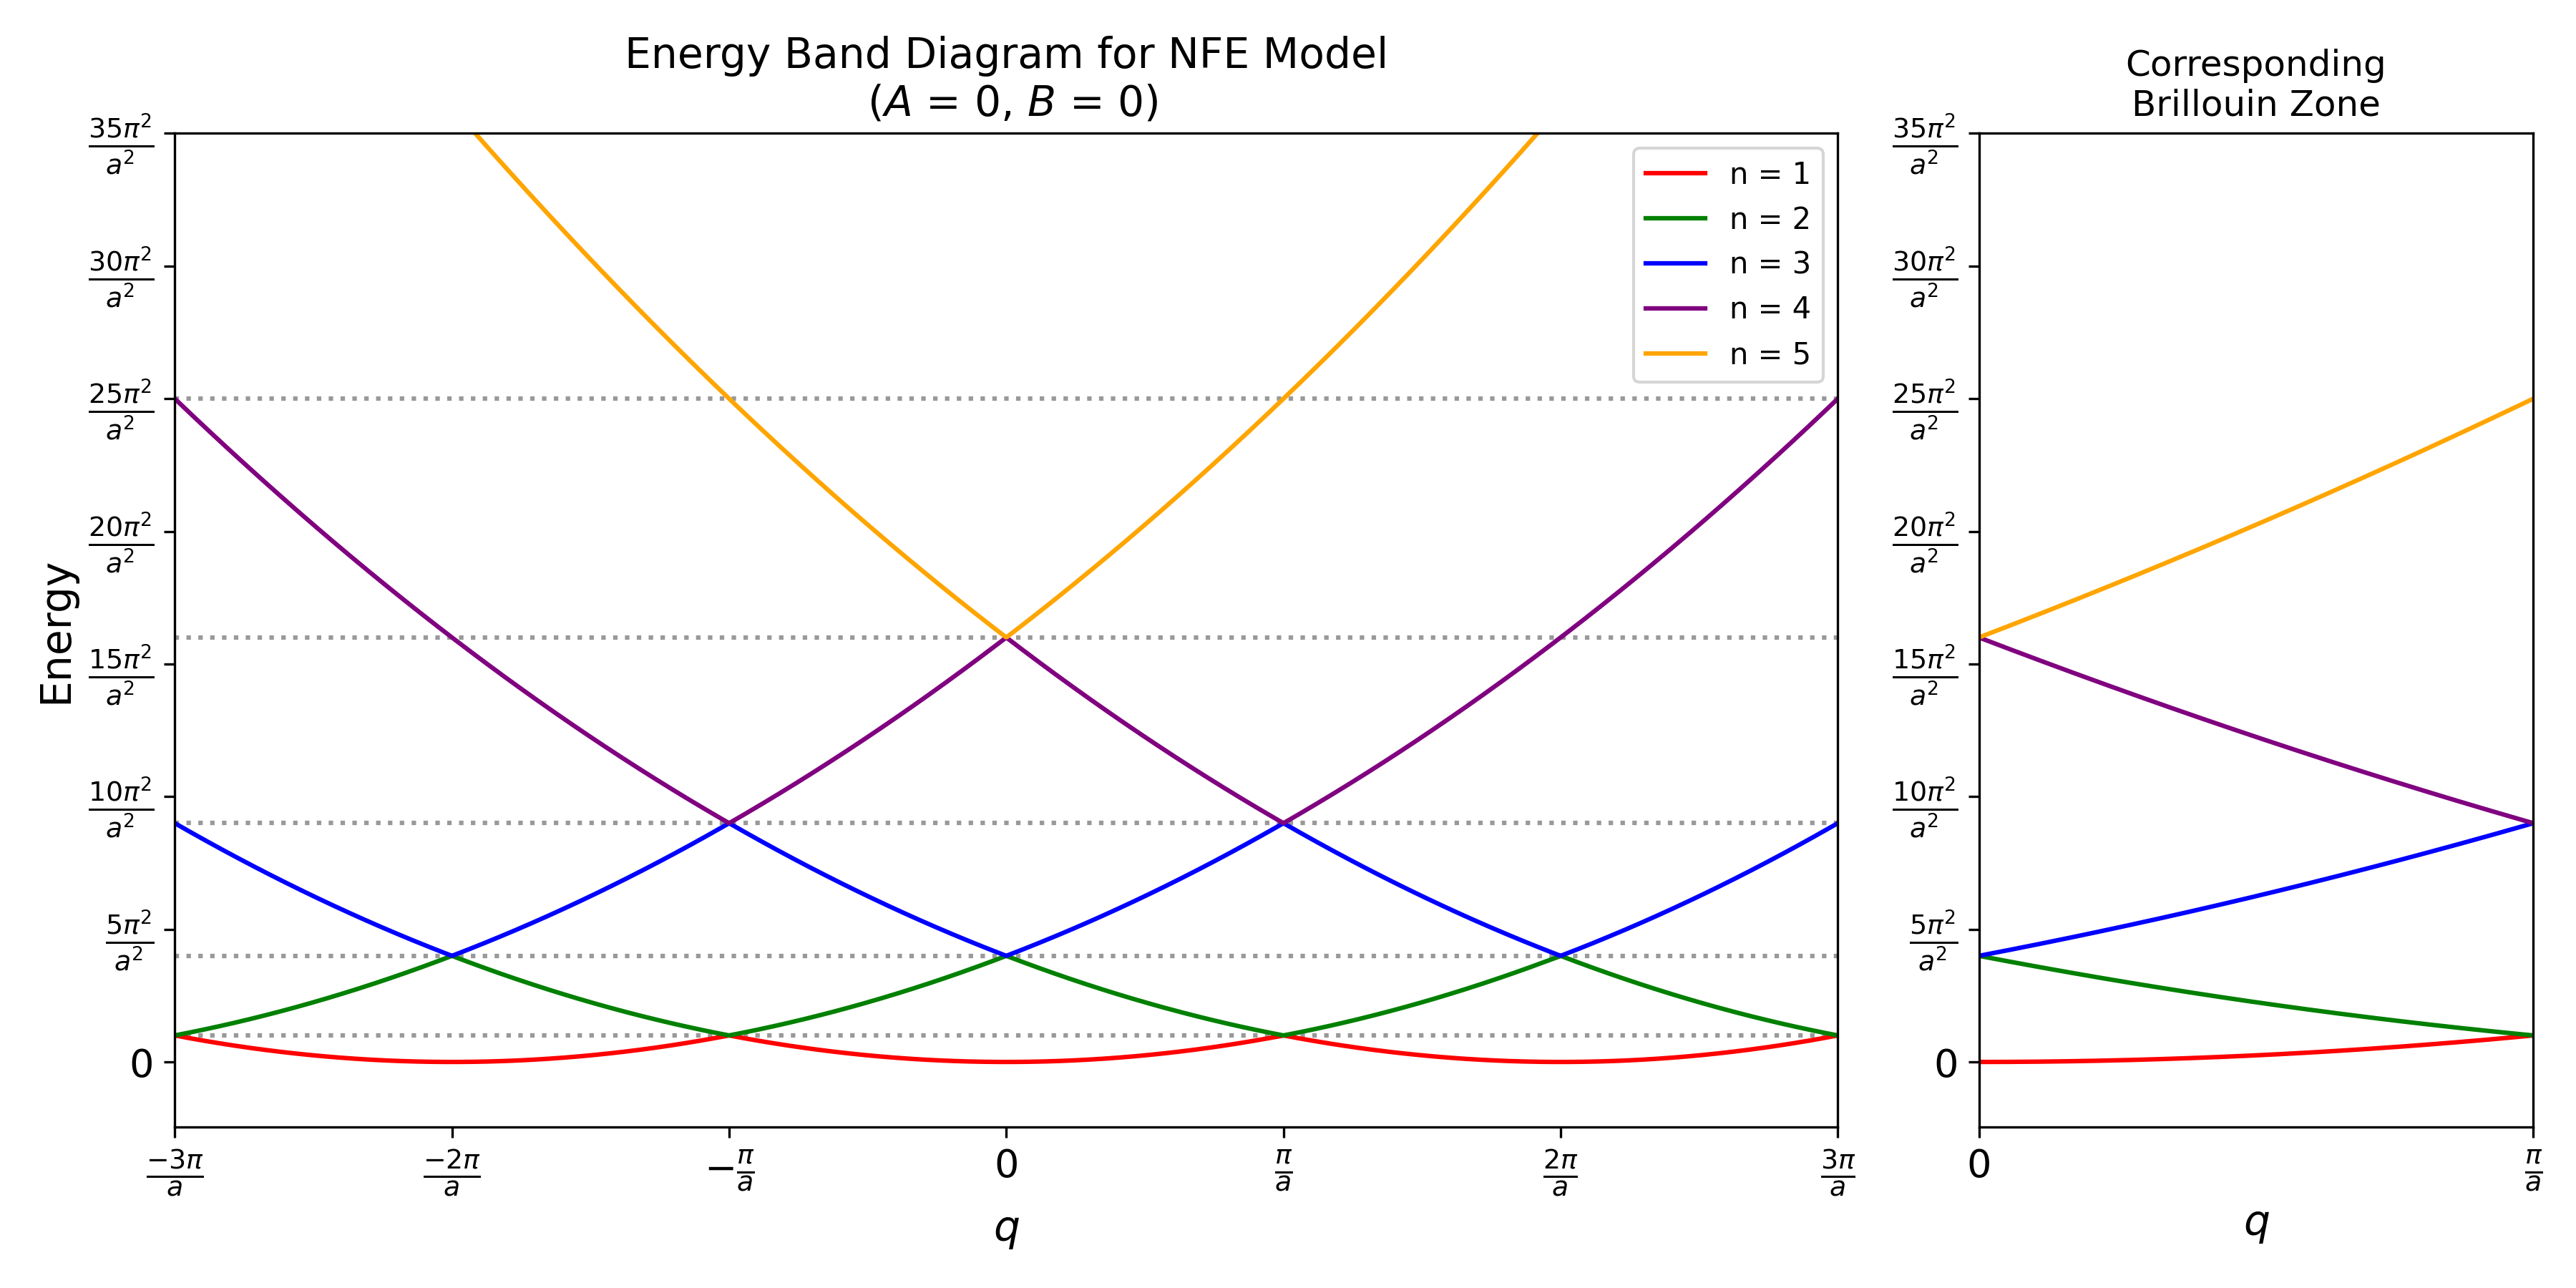
\includegraphics[width=1\linewidth]{images/1.png}
    \caption{Band Structure for when $A=0$ and $B=0$, i.e. a free electron.}
    \label{1}
\end{figure}

\begin{figure}[H]
    \centering
    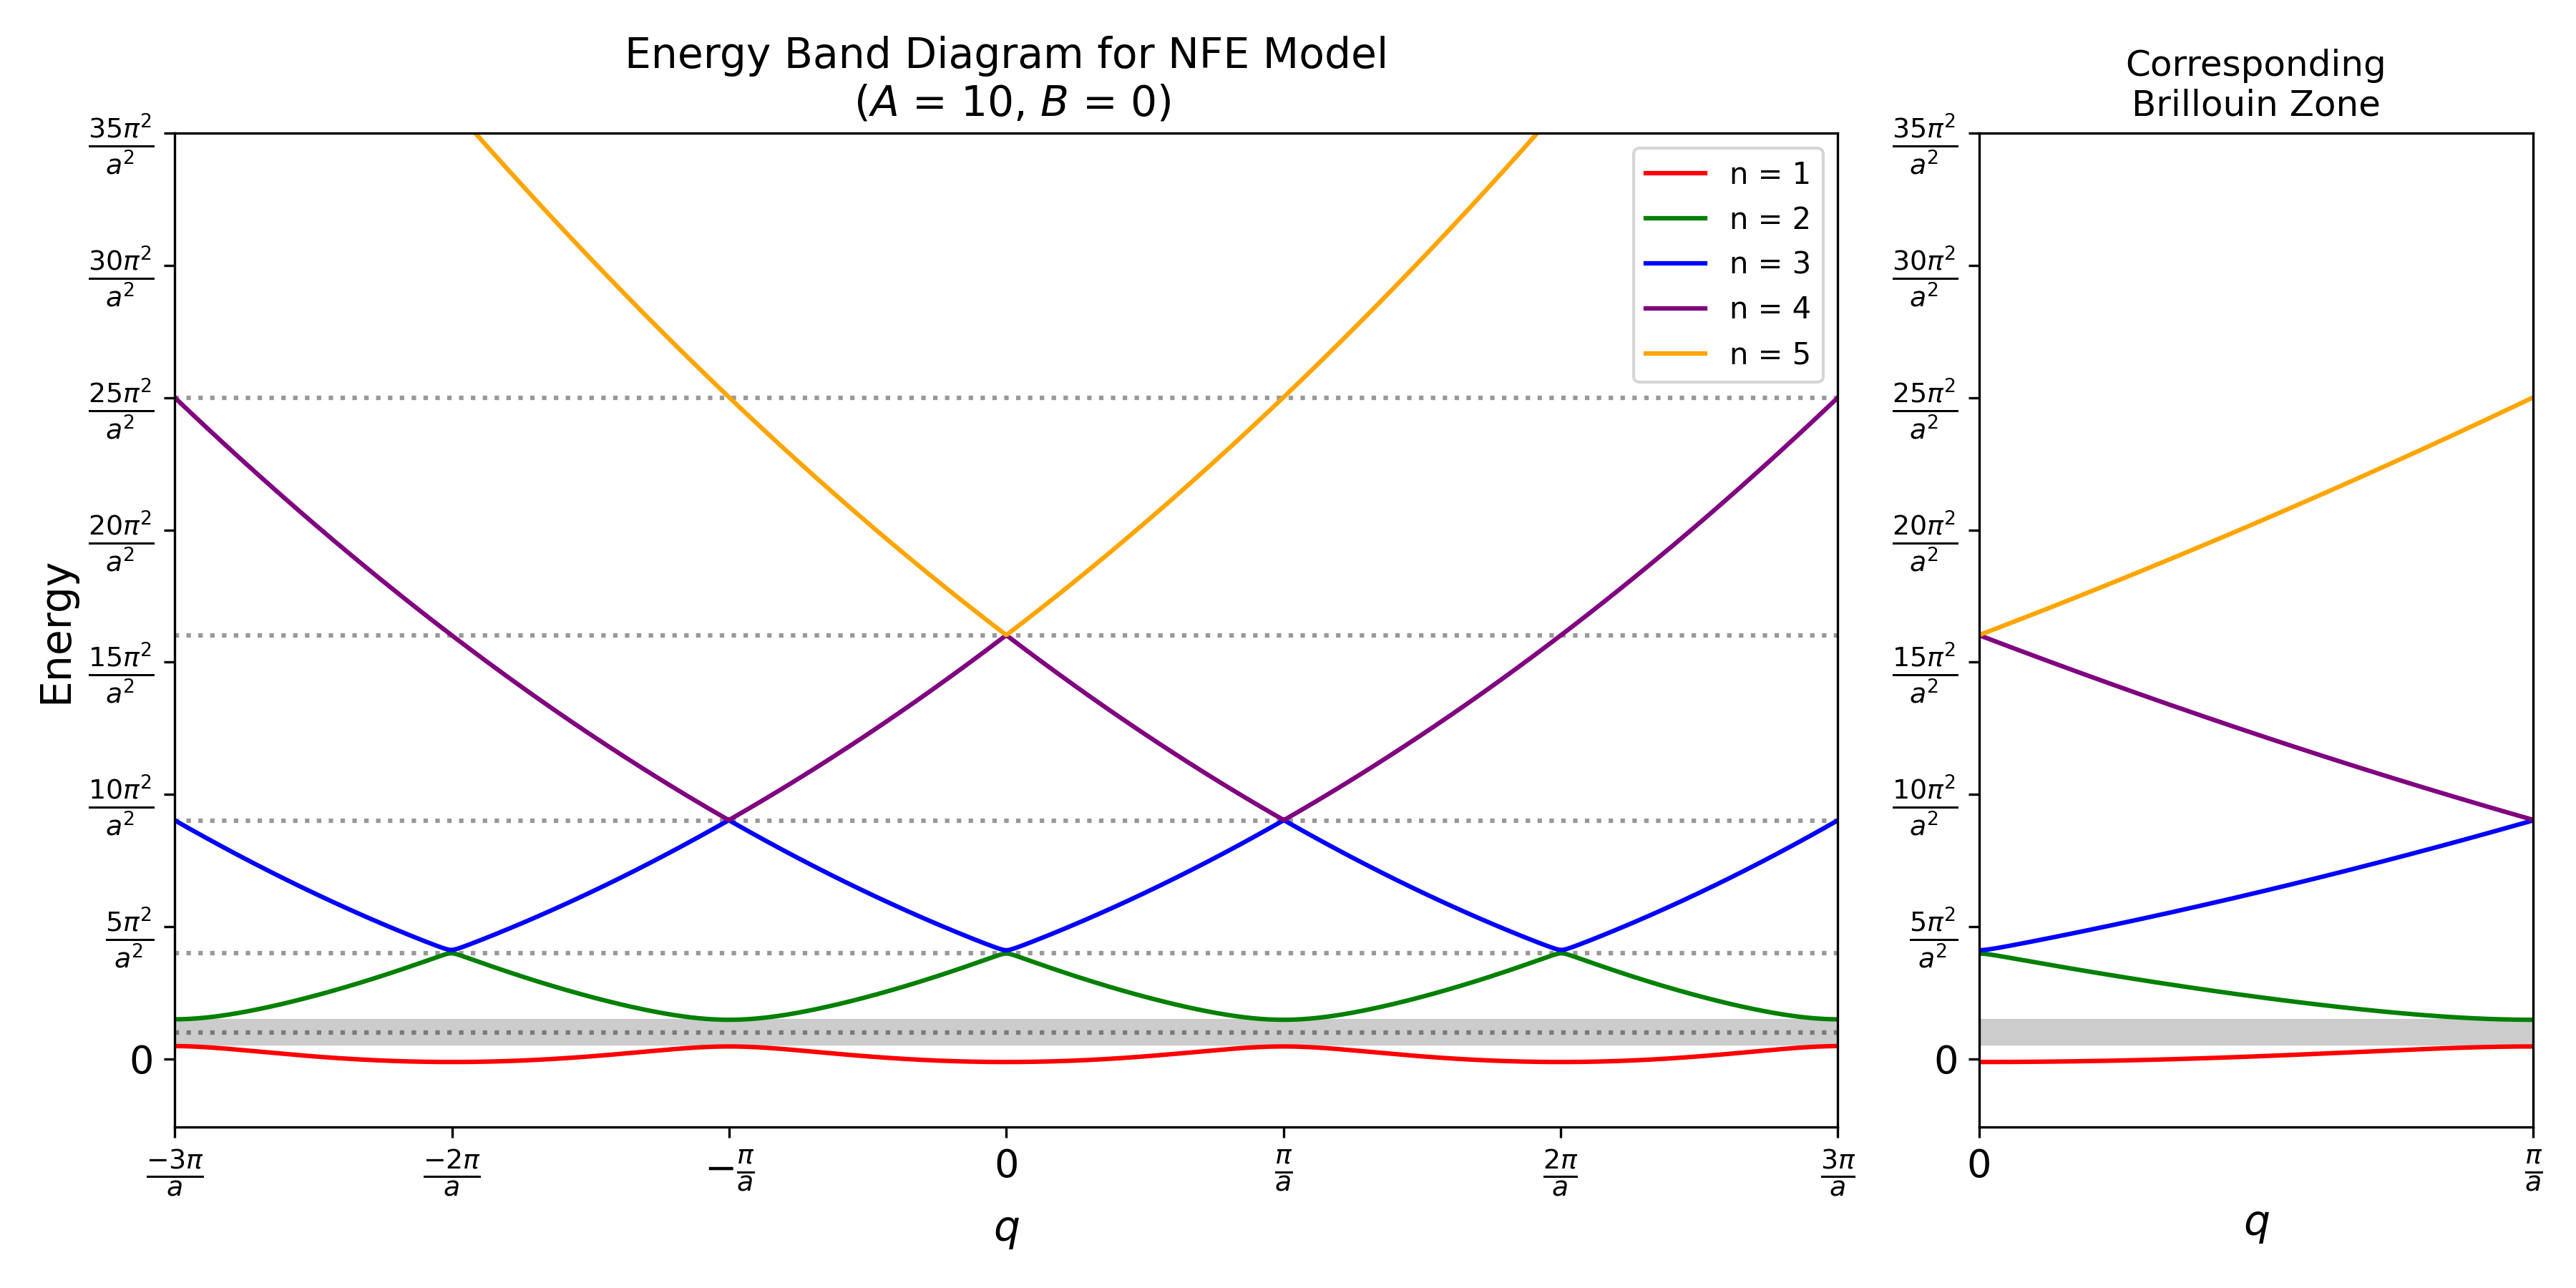
\includegraphics[width=1\linewidth]{images/2.png}
    \caption{Band Structure for when $A=10$ and $B=0$. As you can see, this opens up a gap between the first and second bands at $q=\pi/a$ in the Brillouin zone, of magnitude $A$. The energy gap has been highlighted in the plot.}
    \label{2}
\end{figure}

\begin{figure}[H]
    \centering
    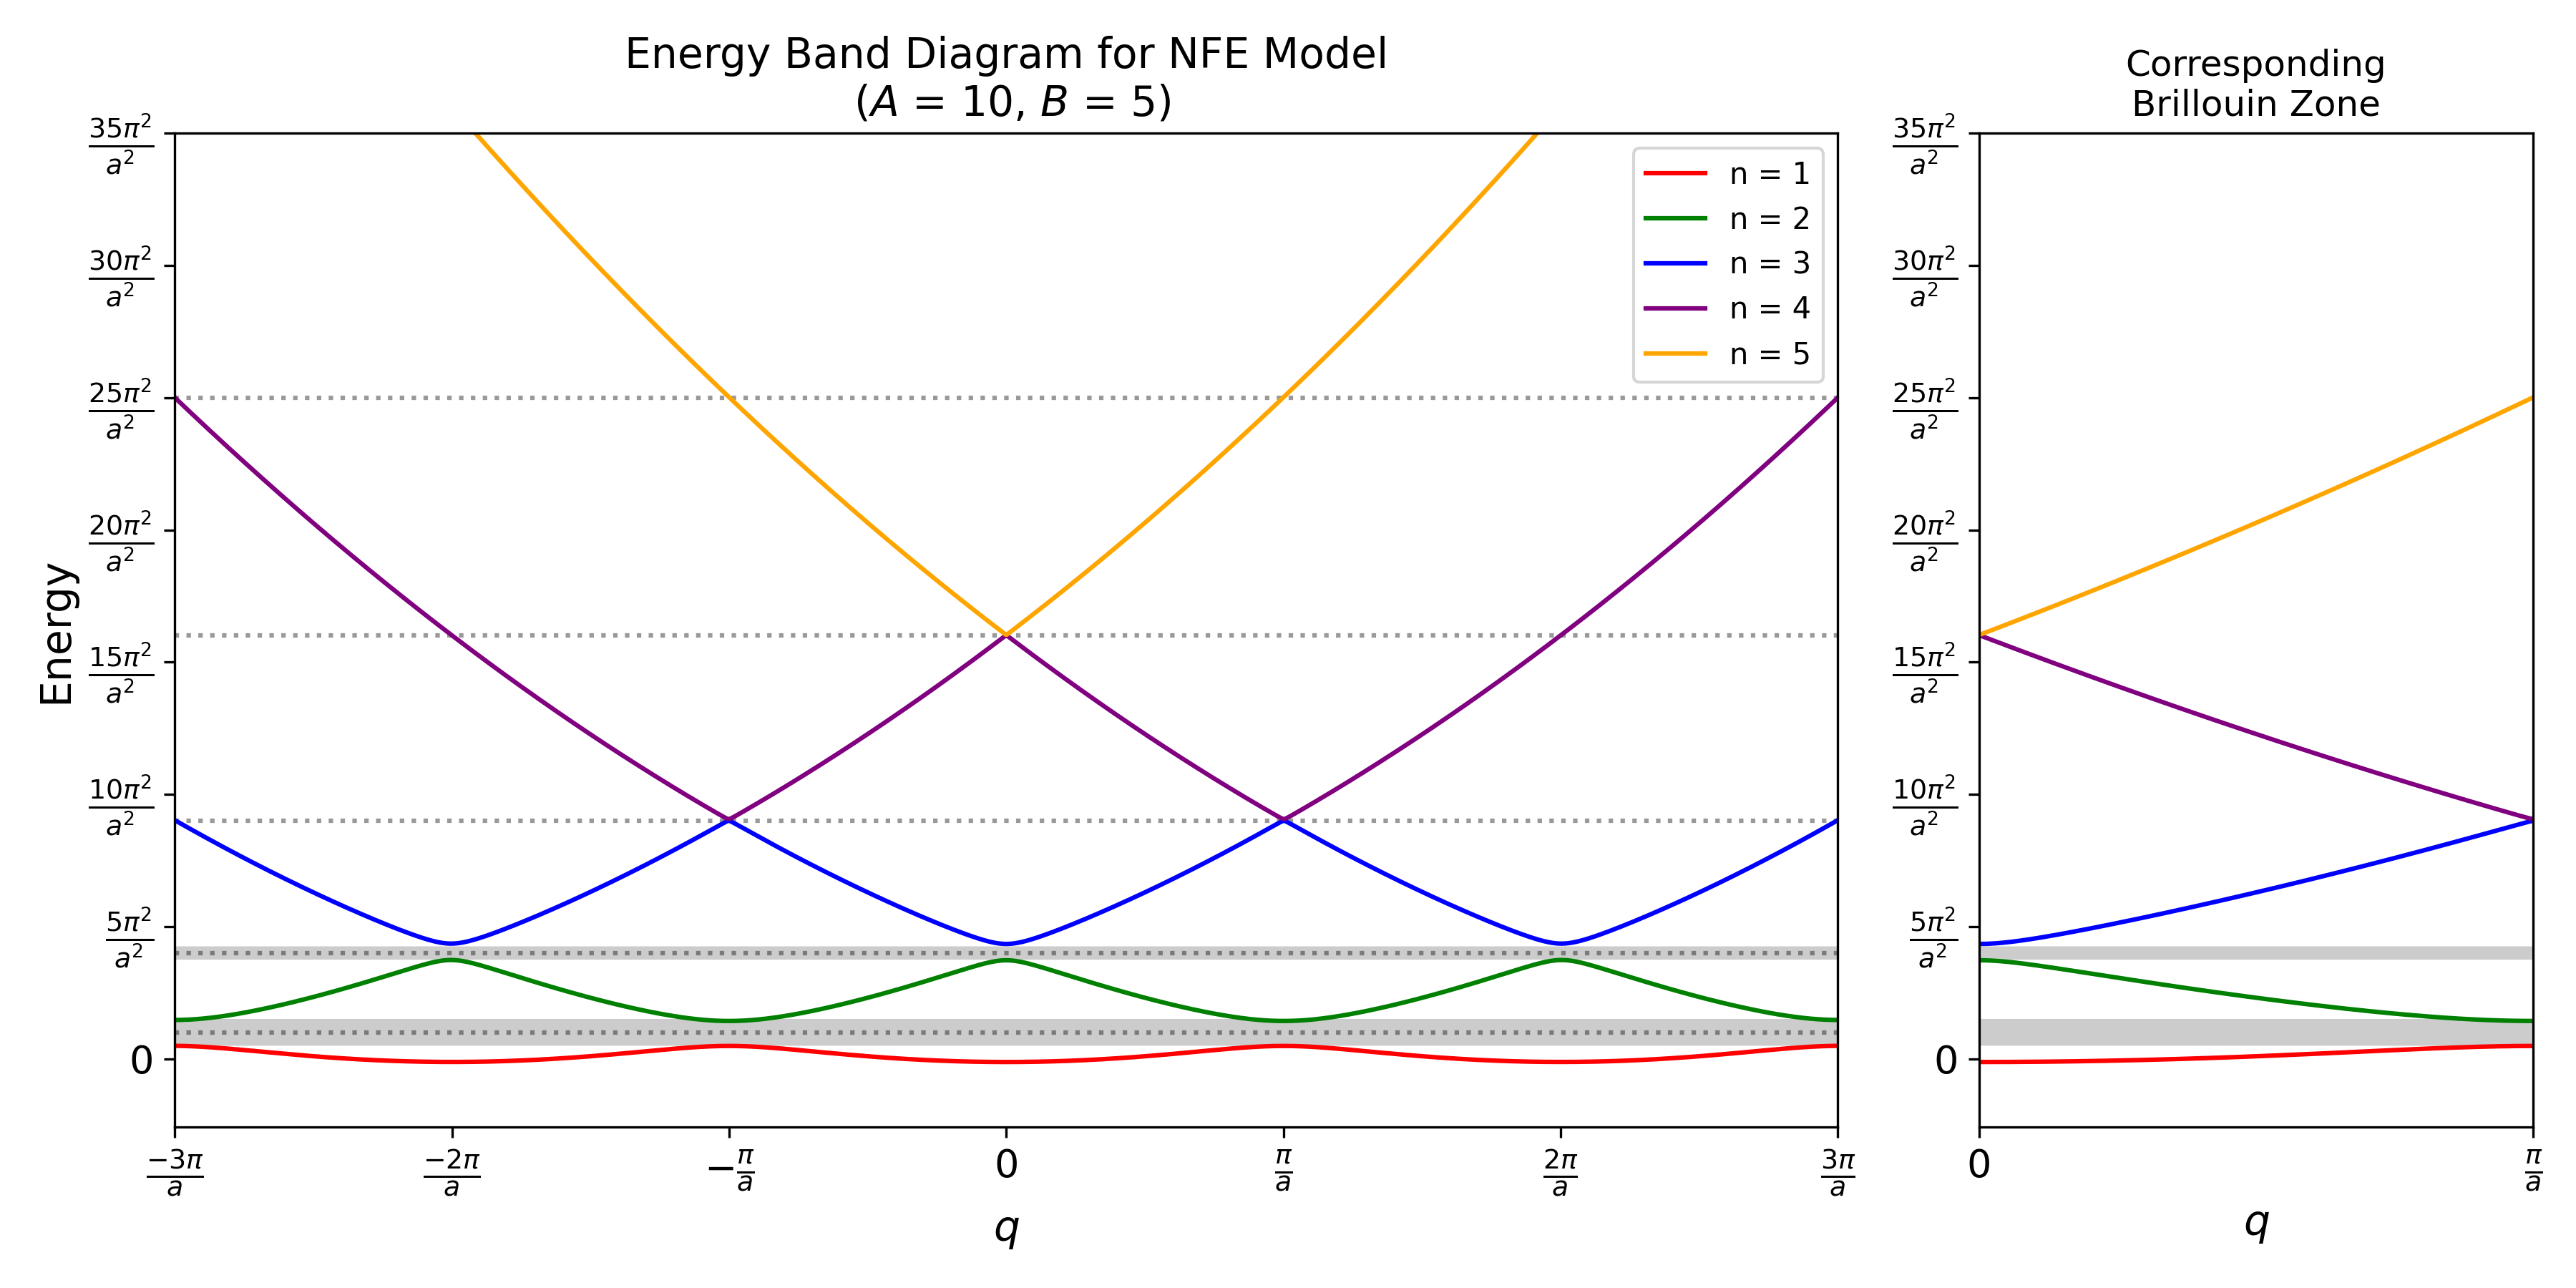
\includegraphics[width=1\linewidth]{images/3.png}
    \caption{Band Structure for when $A=10$ and $B=5$. As you can see, this opens up a gap between the first and second bands at $q=\pi/a$ in the Brillouin zone, of magnitude $A$, and an energy gap between bands 2 and 3 at $q=0$ of magnitude $B$. The energy gaps have been highlighted in the plot.}
    \label{3}
\end{figure}

\begin{figure}[H]
    \centering
    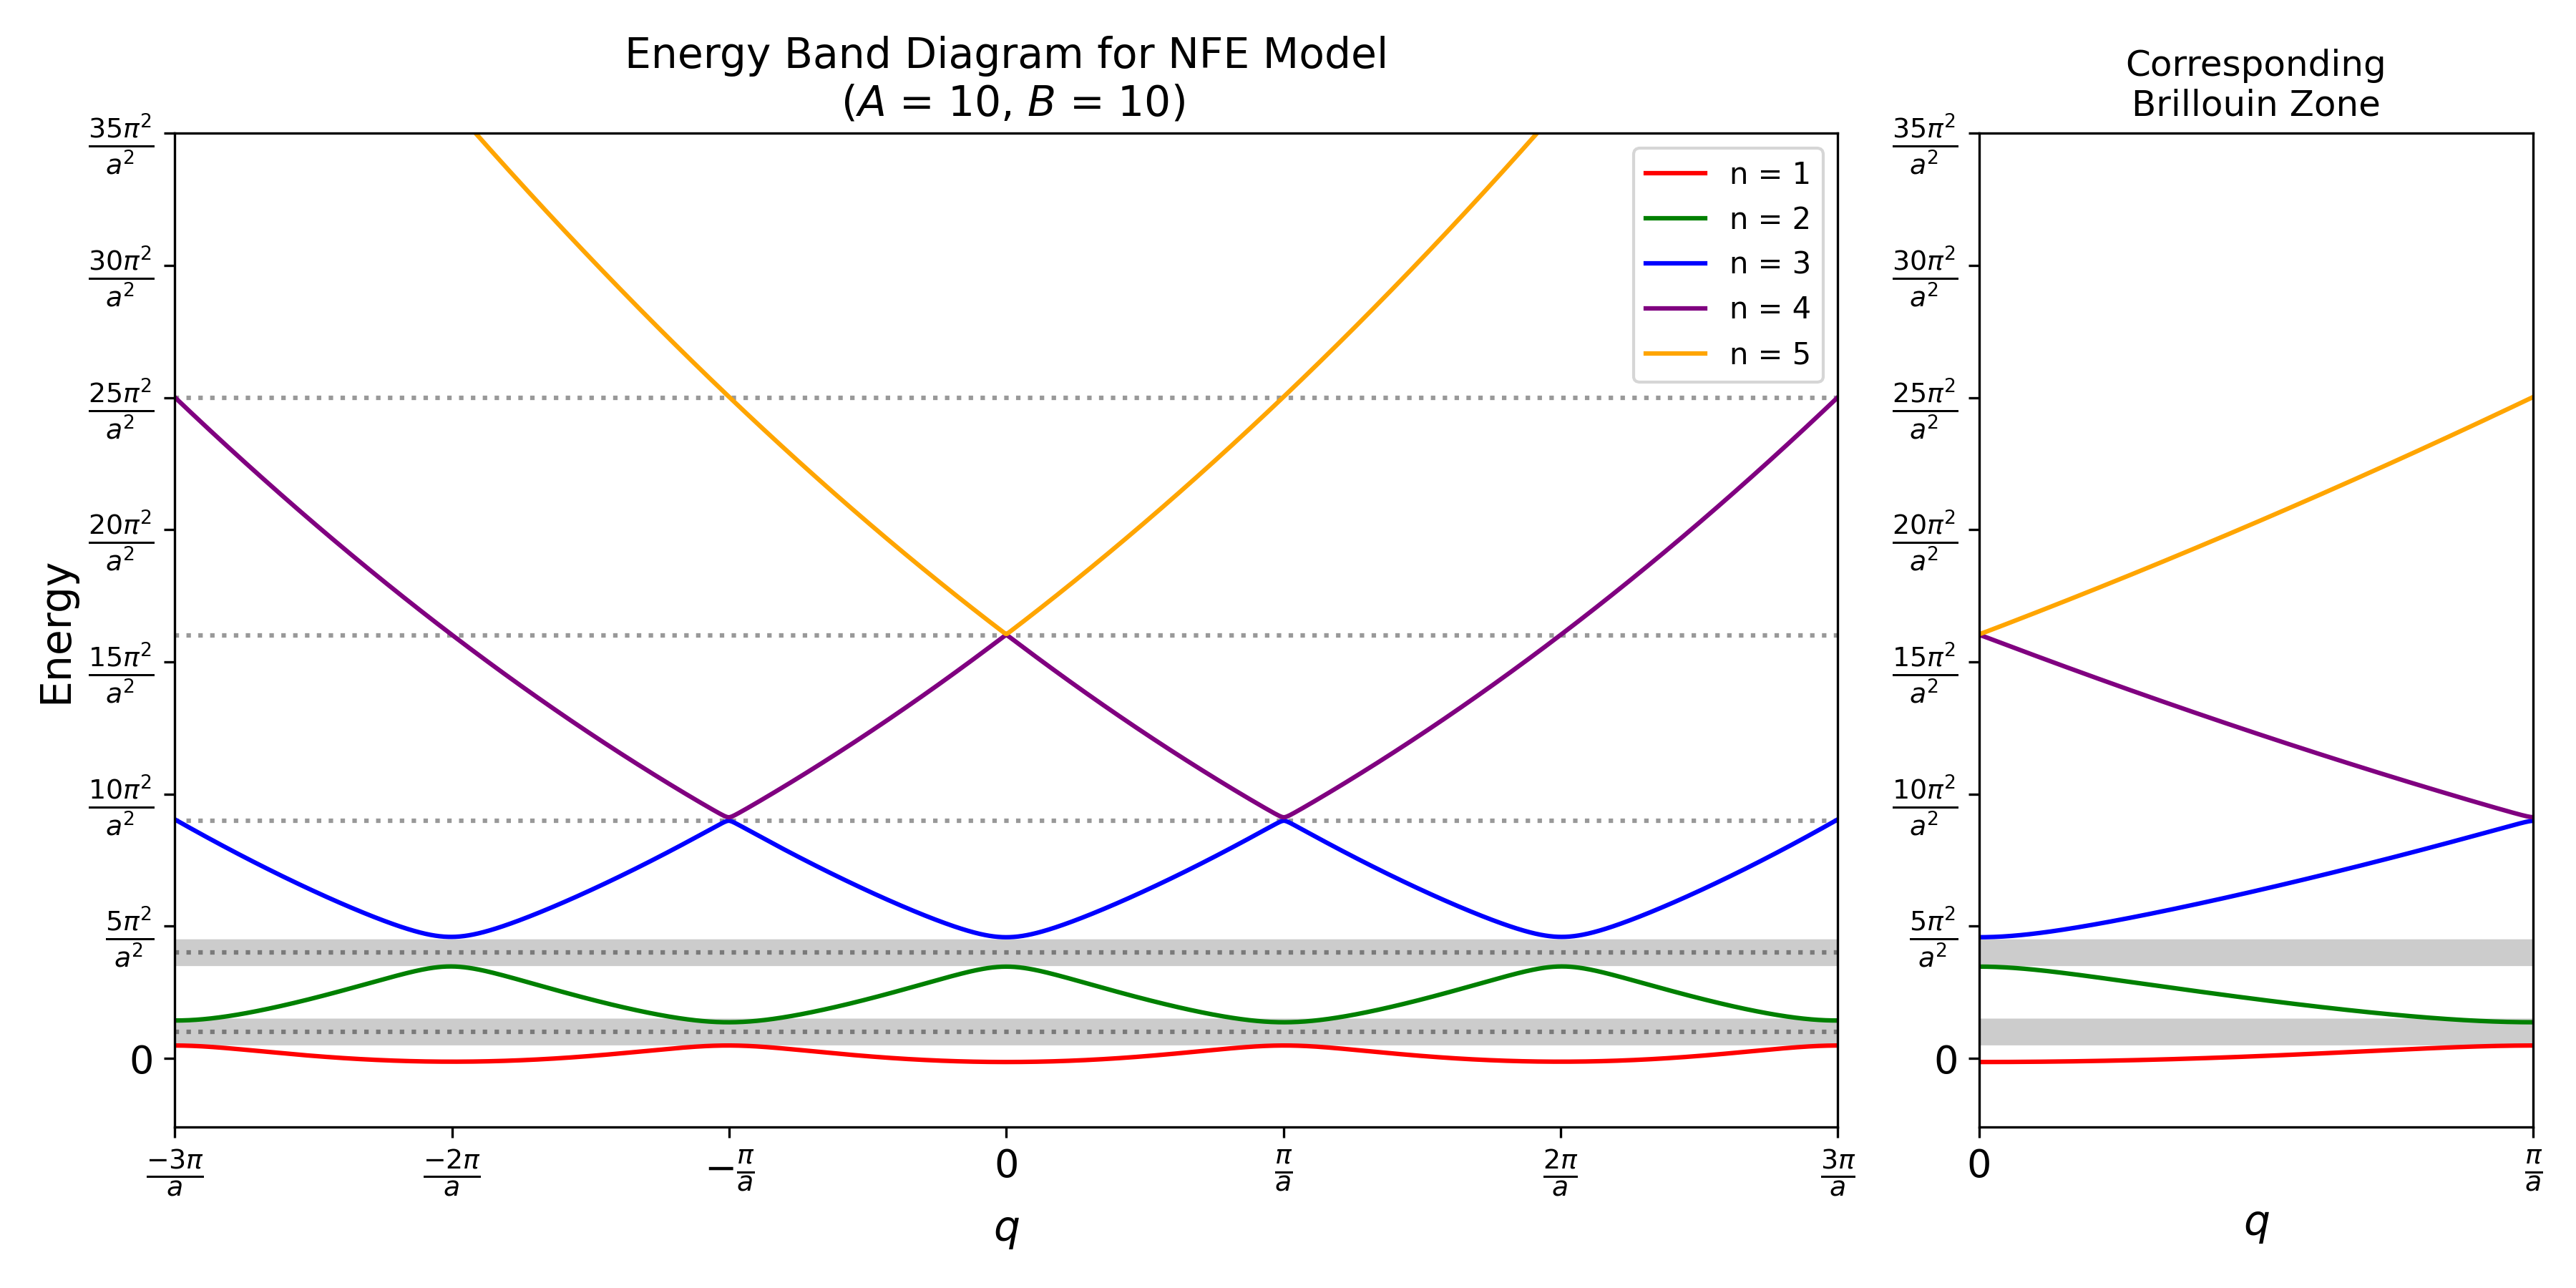
\includegraphics[width=1\linewidth]{images/4.png}
    \caption{Band Structure for when $A=10$ and $B=10$. As you can see, this opens up a gap between the first and second bands at $q=\pi/a$ in the Brillouin zone, of magnitude $A$, and an energy gap between bands 2 and 3 at $q=0$ of magnitude $B$. The energy gaps have been highlighted in the plot.}
    \label{4}
\end{figure}

\begin{figure}[H]
    \centering
    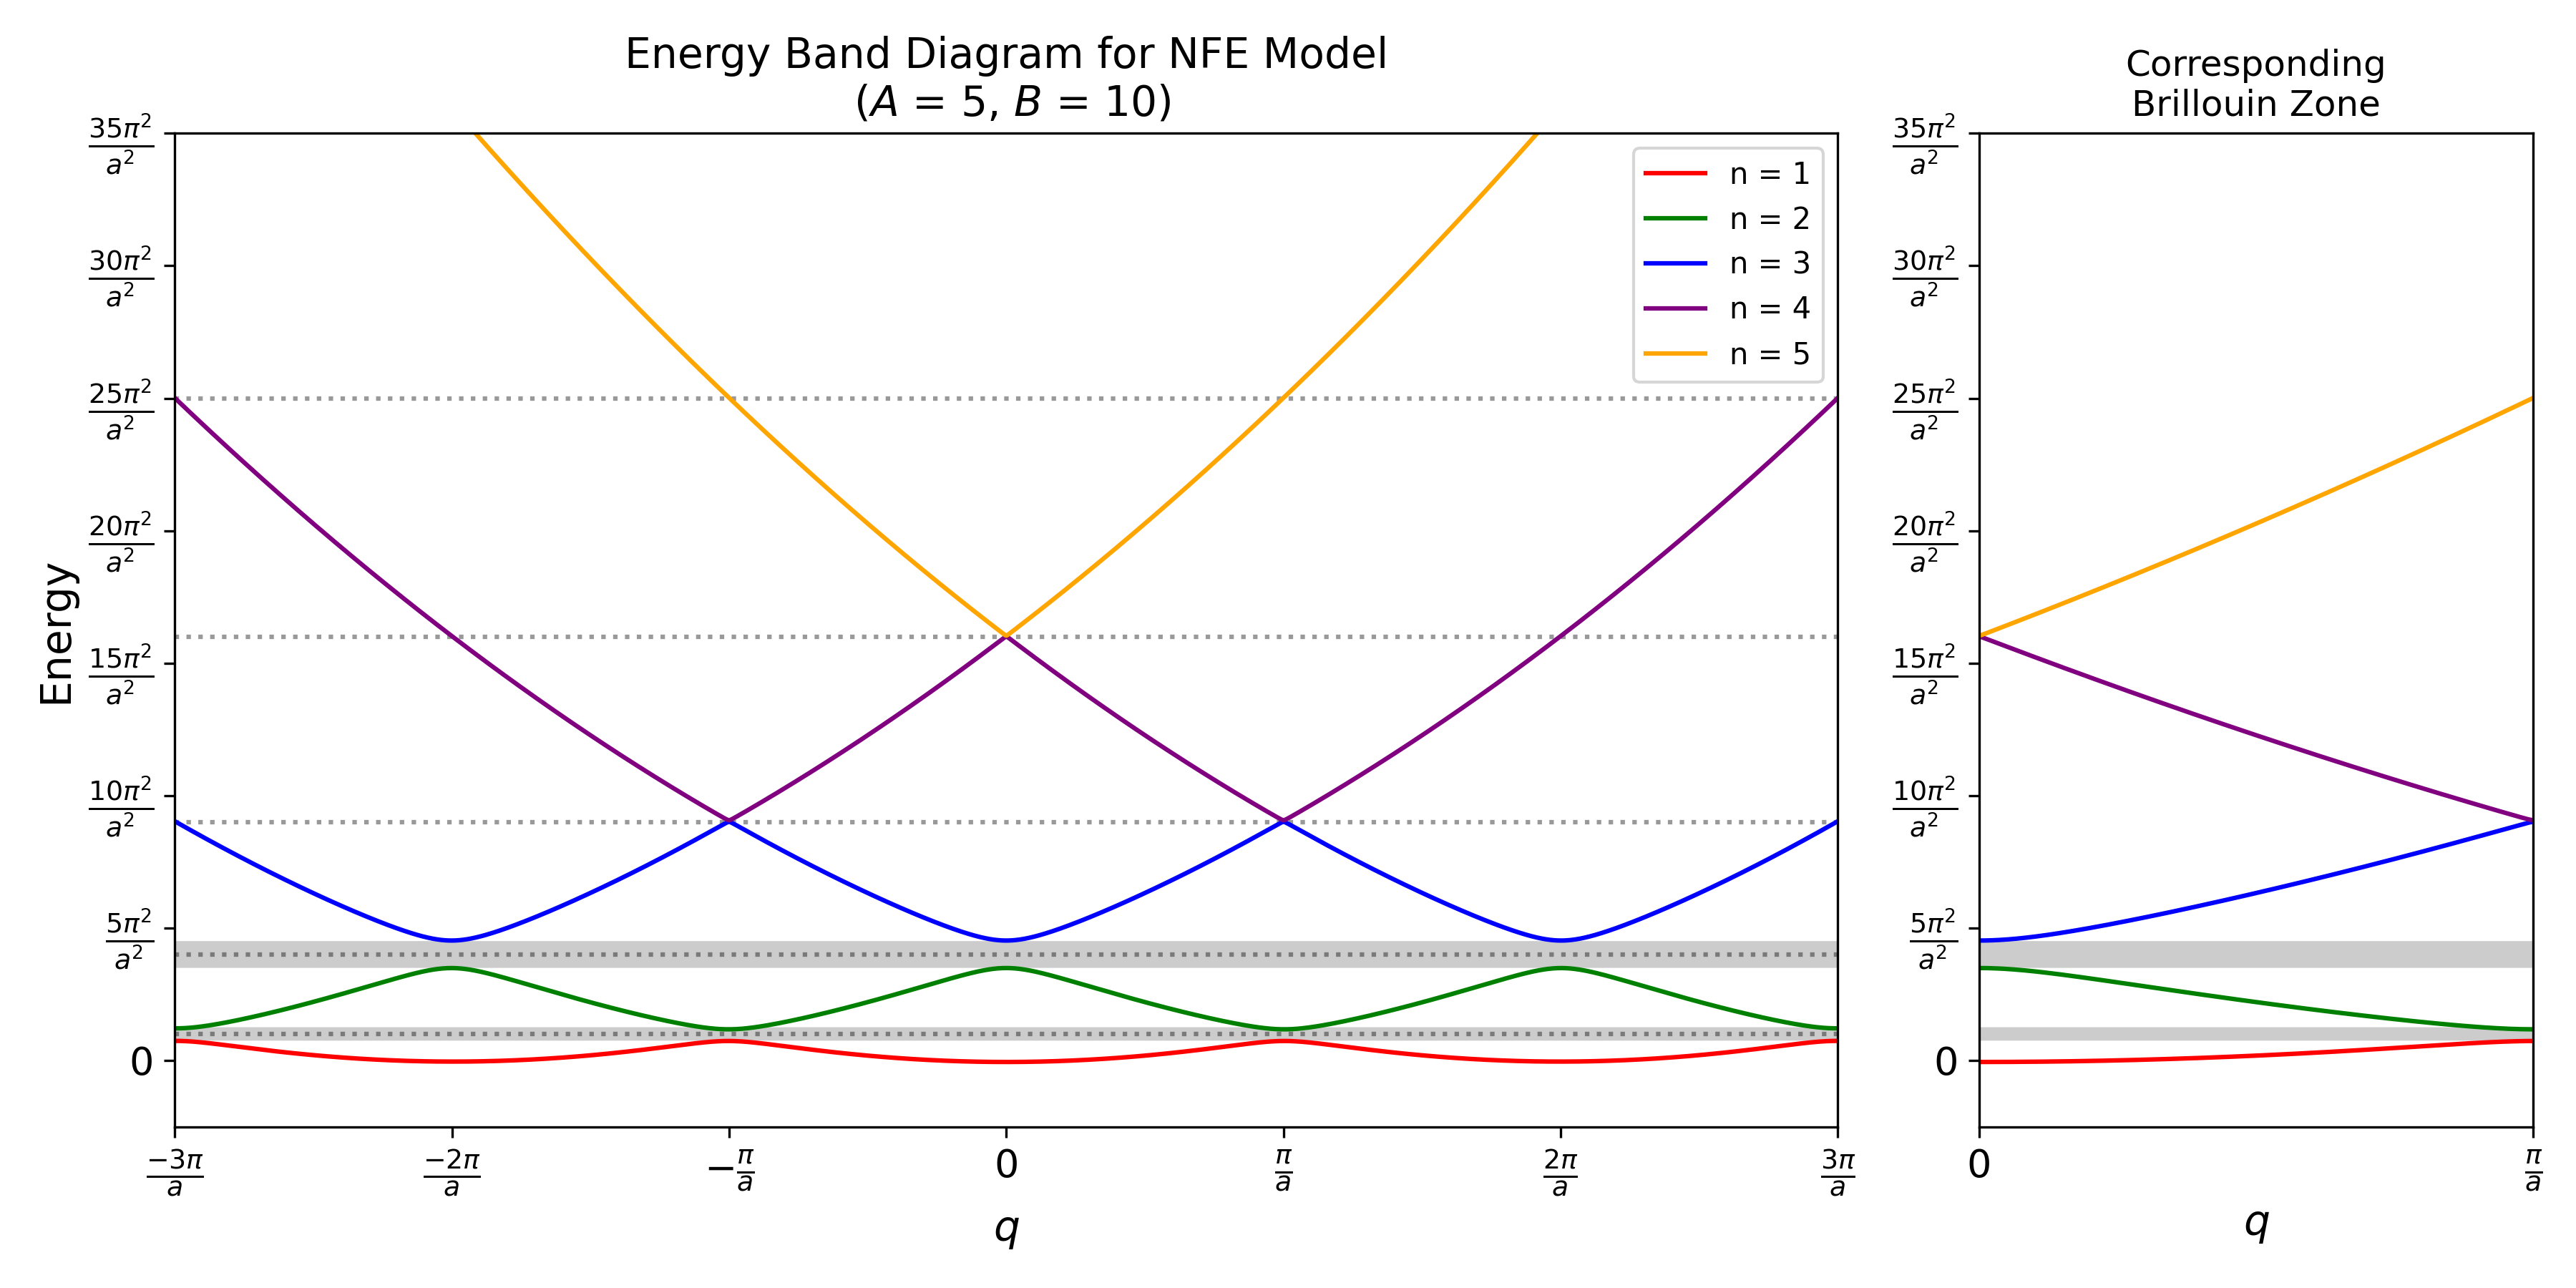
\includegraphics[width=1\linewidth]{images/5.png}
    \caption{Band Structure for when $A=5$ and $B=10$. As you can see, this opens up a gap between the first and second bands at $q=\pi/a$ in the Brillouin zone, of magnitude $A$, and an energy gap between bands 2 and 3 at $q=0$ of magnitude $B$. The energy gaps have been highlighted in the plot.}
    \label{5}
\end{figure}

\begin{figure}[H]
    \centering
    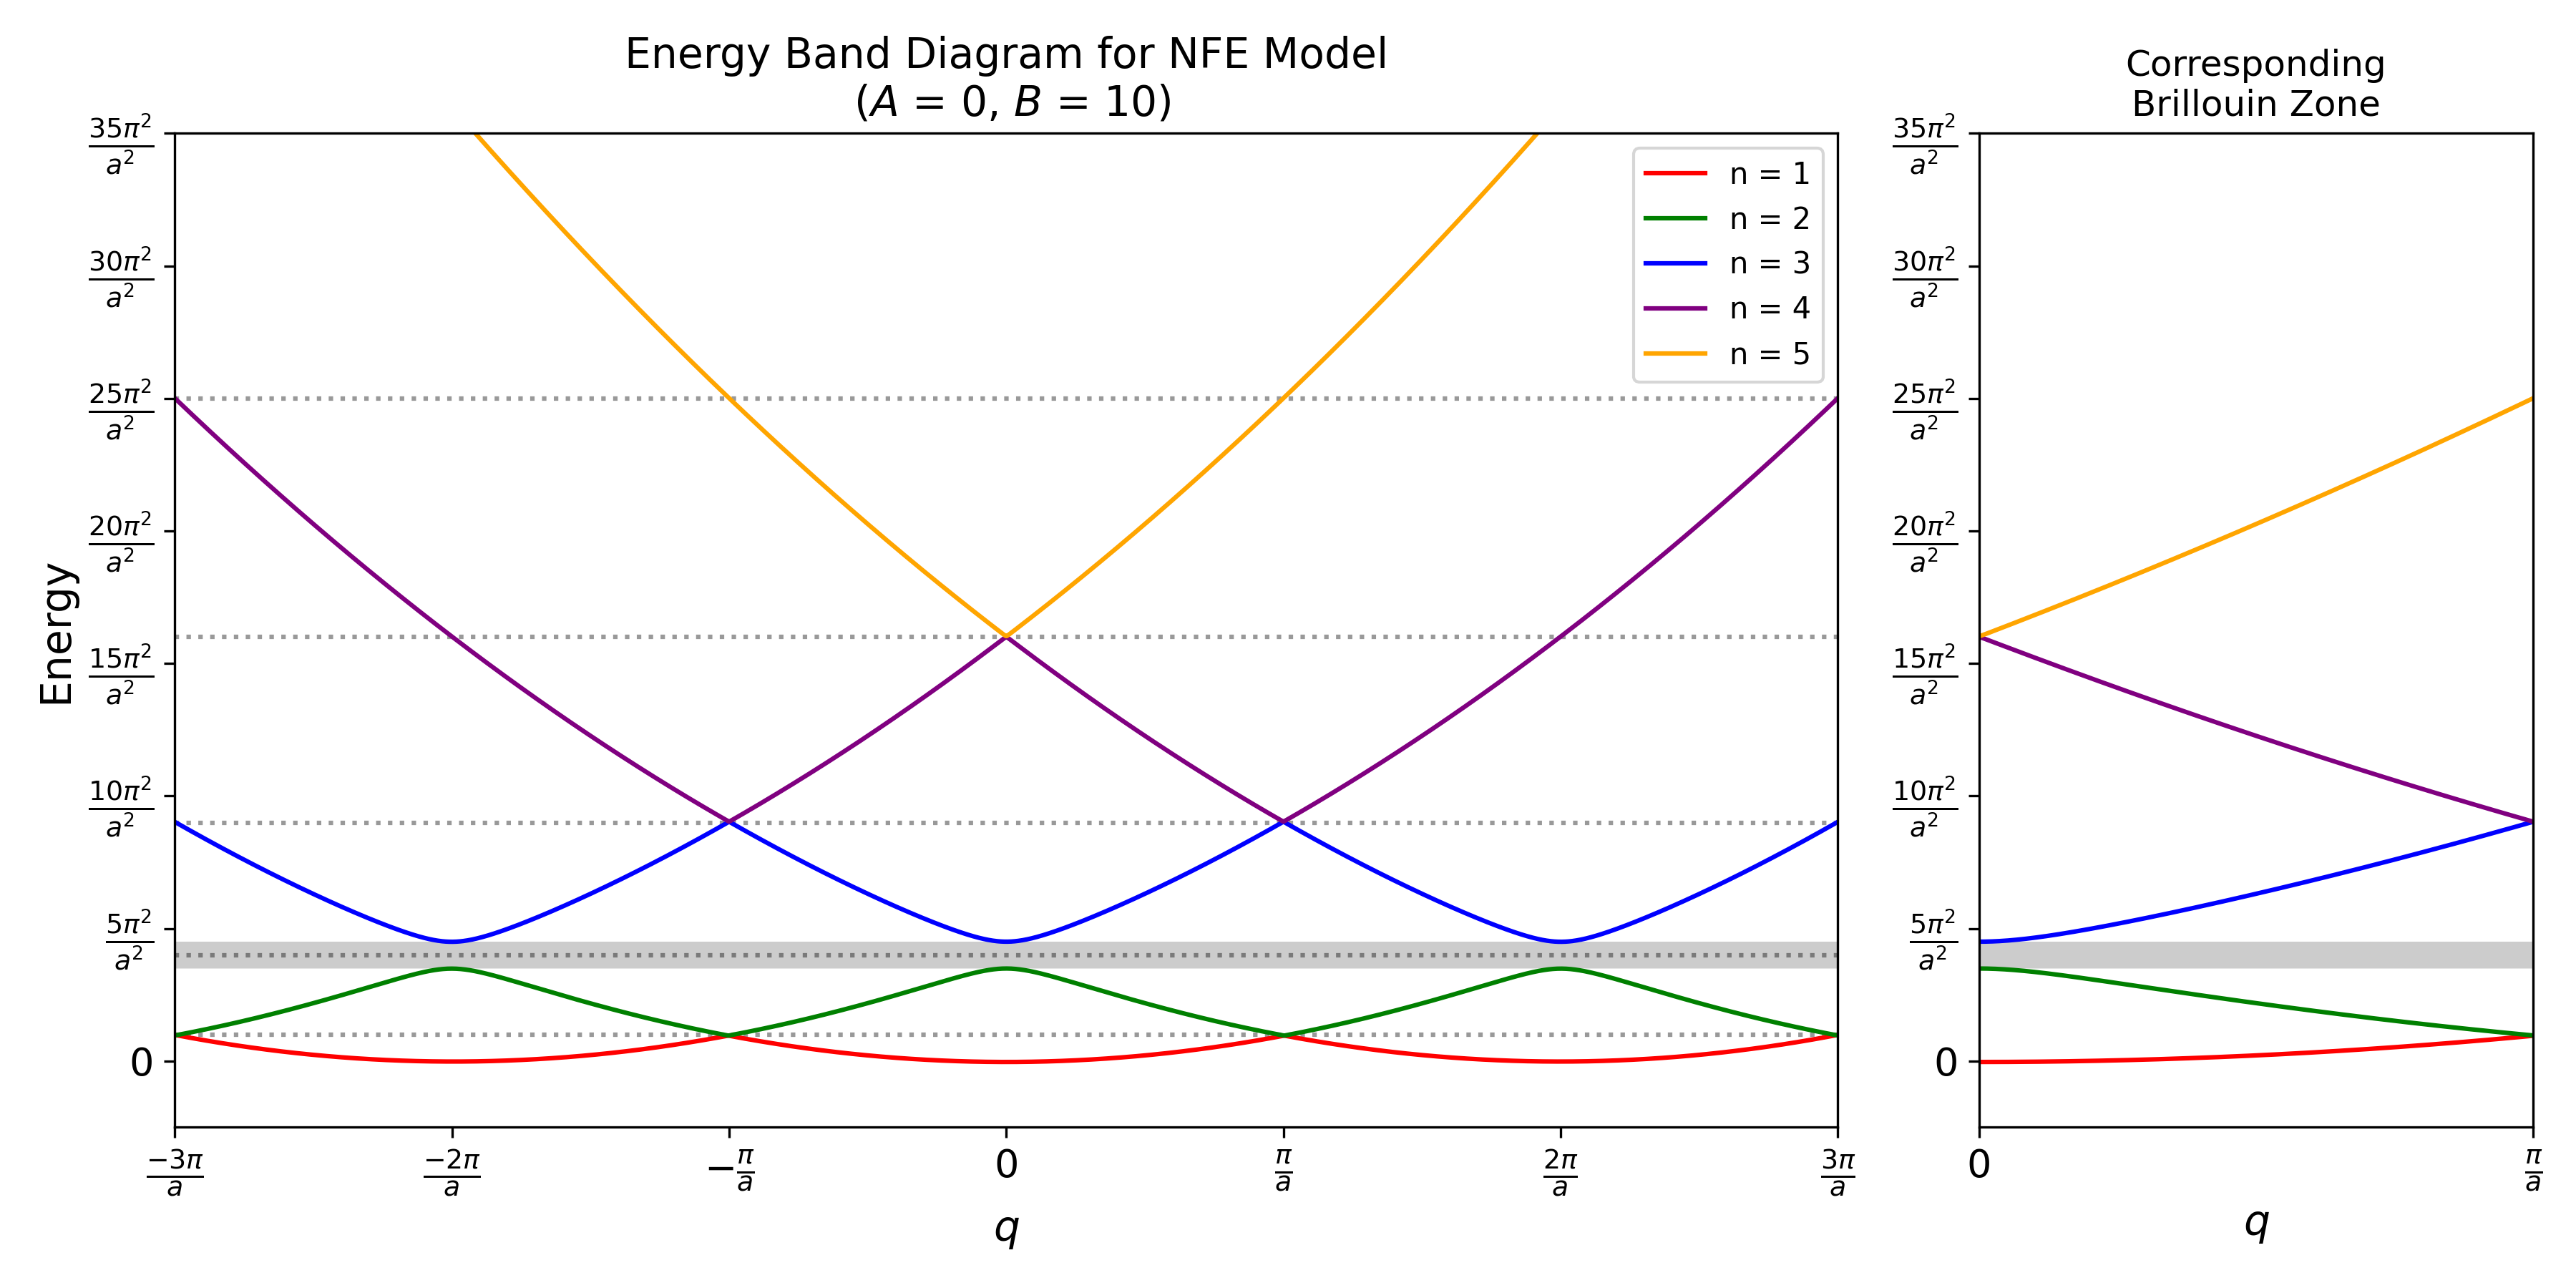
\includegraphics[width=1\linewidth]{images/6.png}
    \caption{Band Structure for when $A=0$ and $B=10$. As you can see, this opens up a gap between the second and third bands at $q=0$ in the Brillouin zone, of magnitude $B$. The energy gaps have been highlighted in the plot.}
    \label{6}
\end{figure}
\subsubsection{For $V > T_q$}

It is to be noted in all these plots that for small values of $A$, the energy gap is only prominent for the first and second bands. However as $A$ increases significantly (beyond their corresponding kinetic energy terms), it leads to a significant band gap in higher bands, but of lesser magnitude, which can be calculated by diagonalising the total Hamiltonian as we see in the following plots.

\begin{figure}[H]
    \centering
    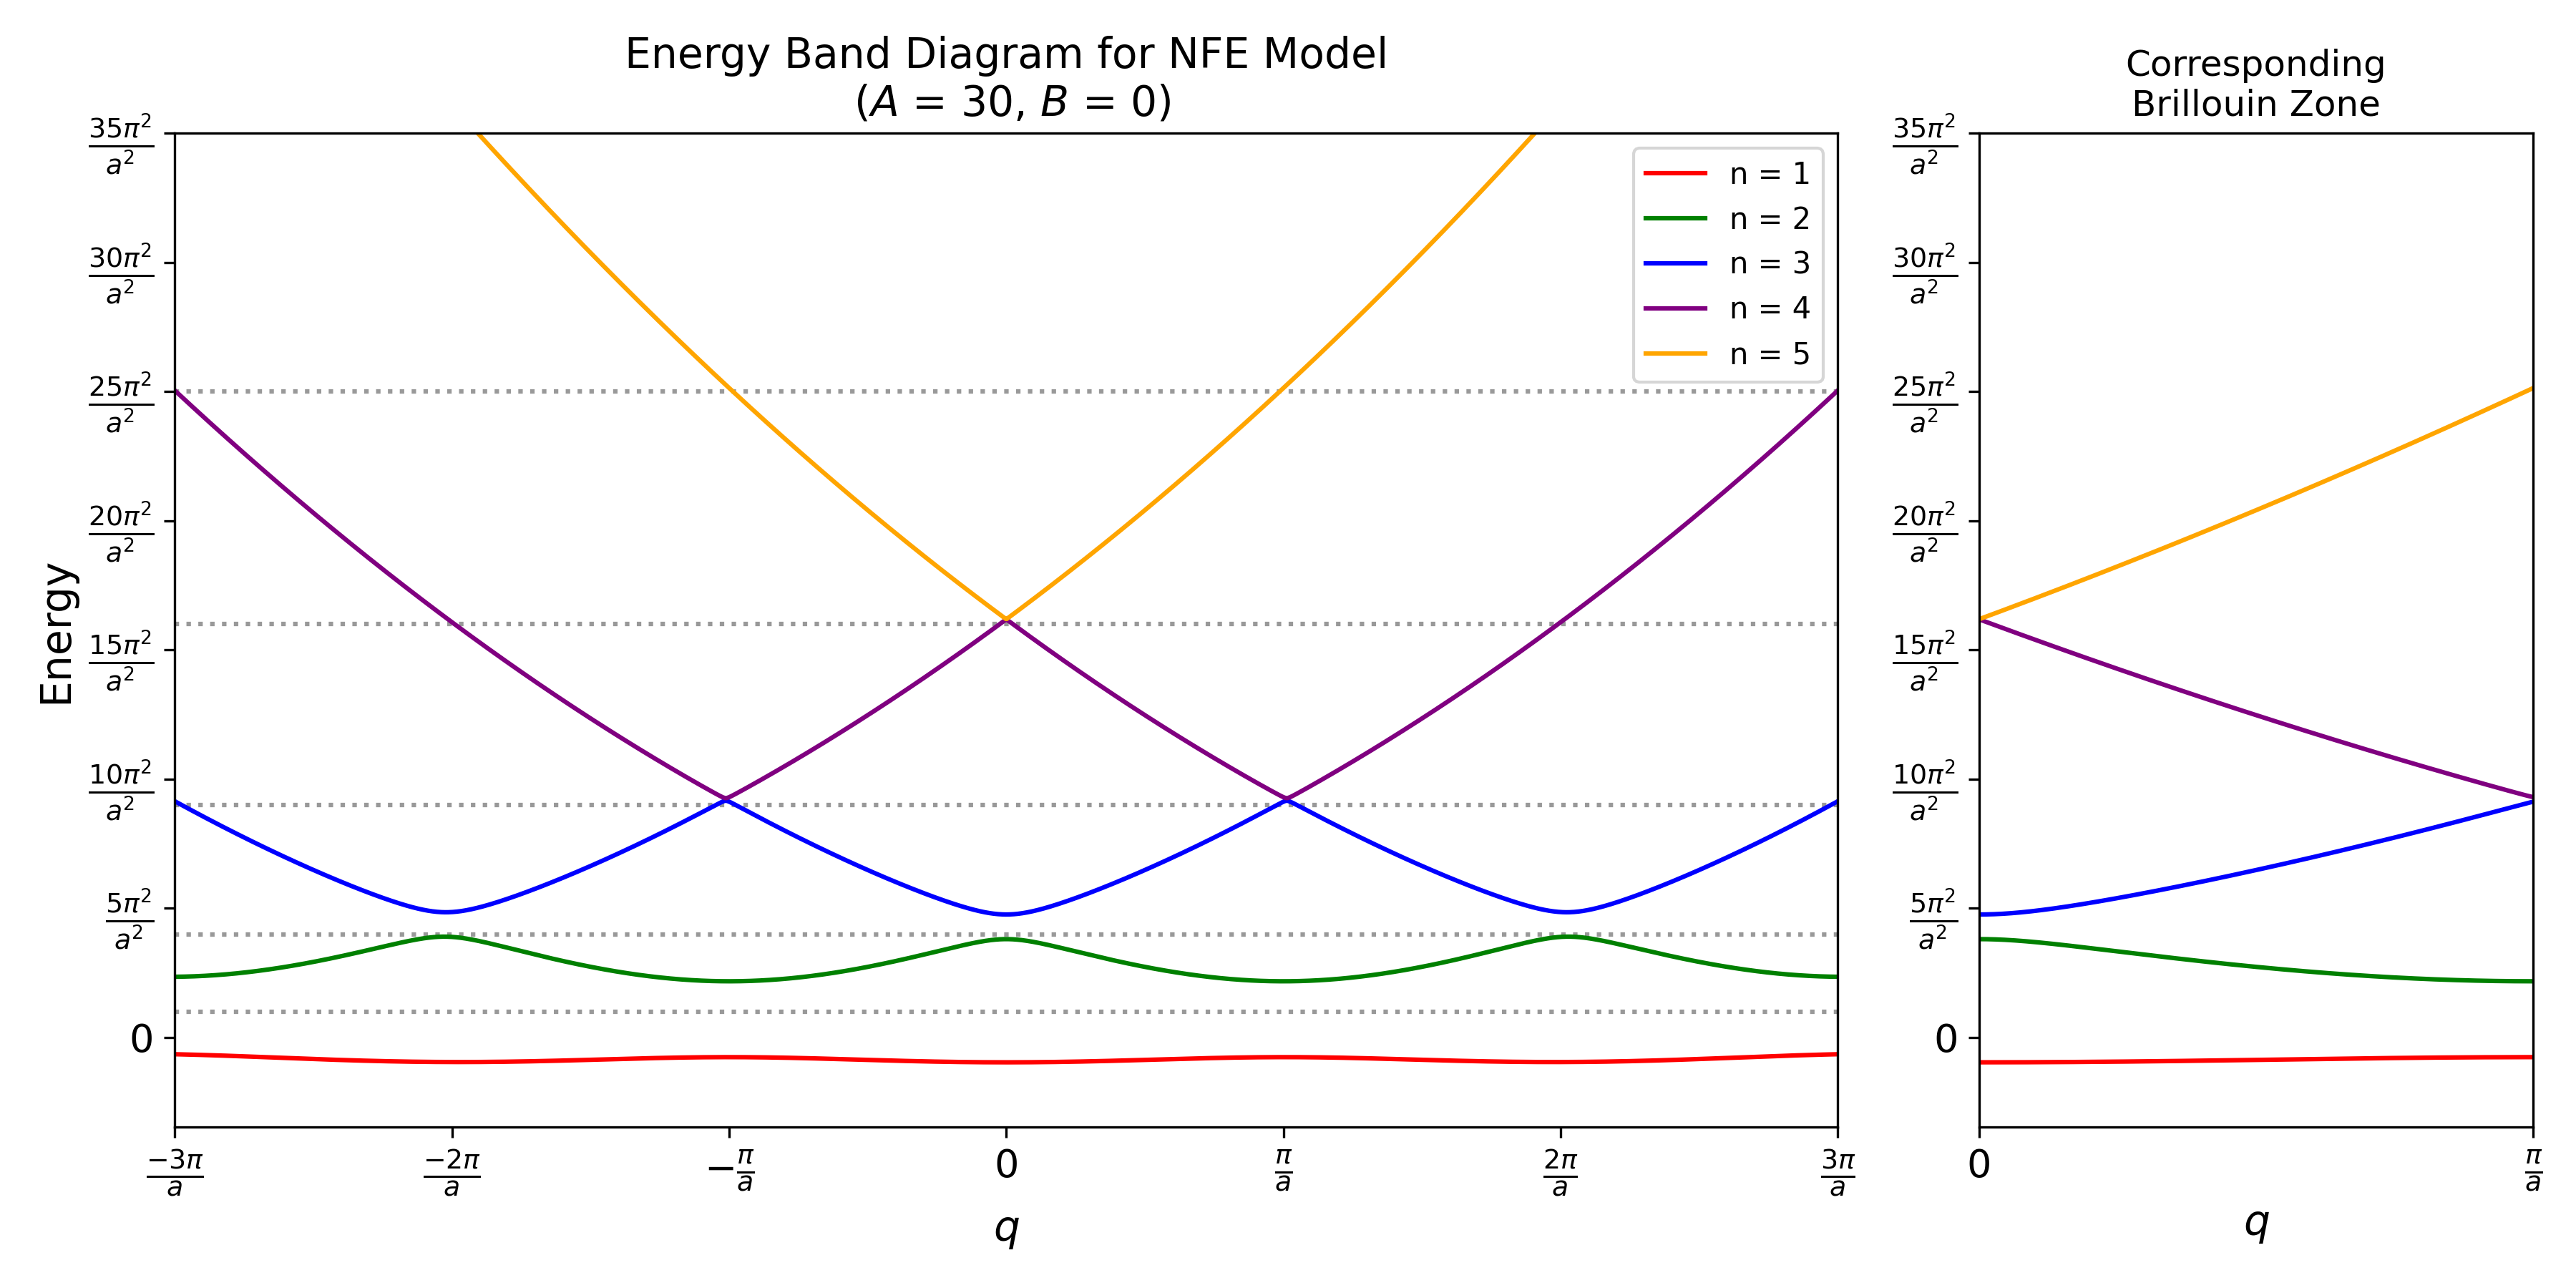
\includegraphics[width=1\linewidth]{images/h1.png}
    \caption{Band Structure for when $A=30$ and $B=0$. As you can see, this opens up a non-zero gap between all the bands in decreasing magnitude.}
    \label{h1}
\end{figure}

Similarly on increasing the $B$ value beyond their corresponding kinetic energy levels, it also opens up a band gap in every other pair higher order bands (i.e. only for $q=0$ in the Brillouin Zone). This is beacuse $B$ corresponds to the second fourier coefficient. The others remain intact.

\begin{figure}[H]
    \centering
    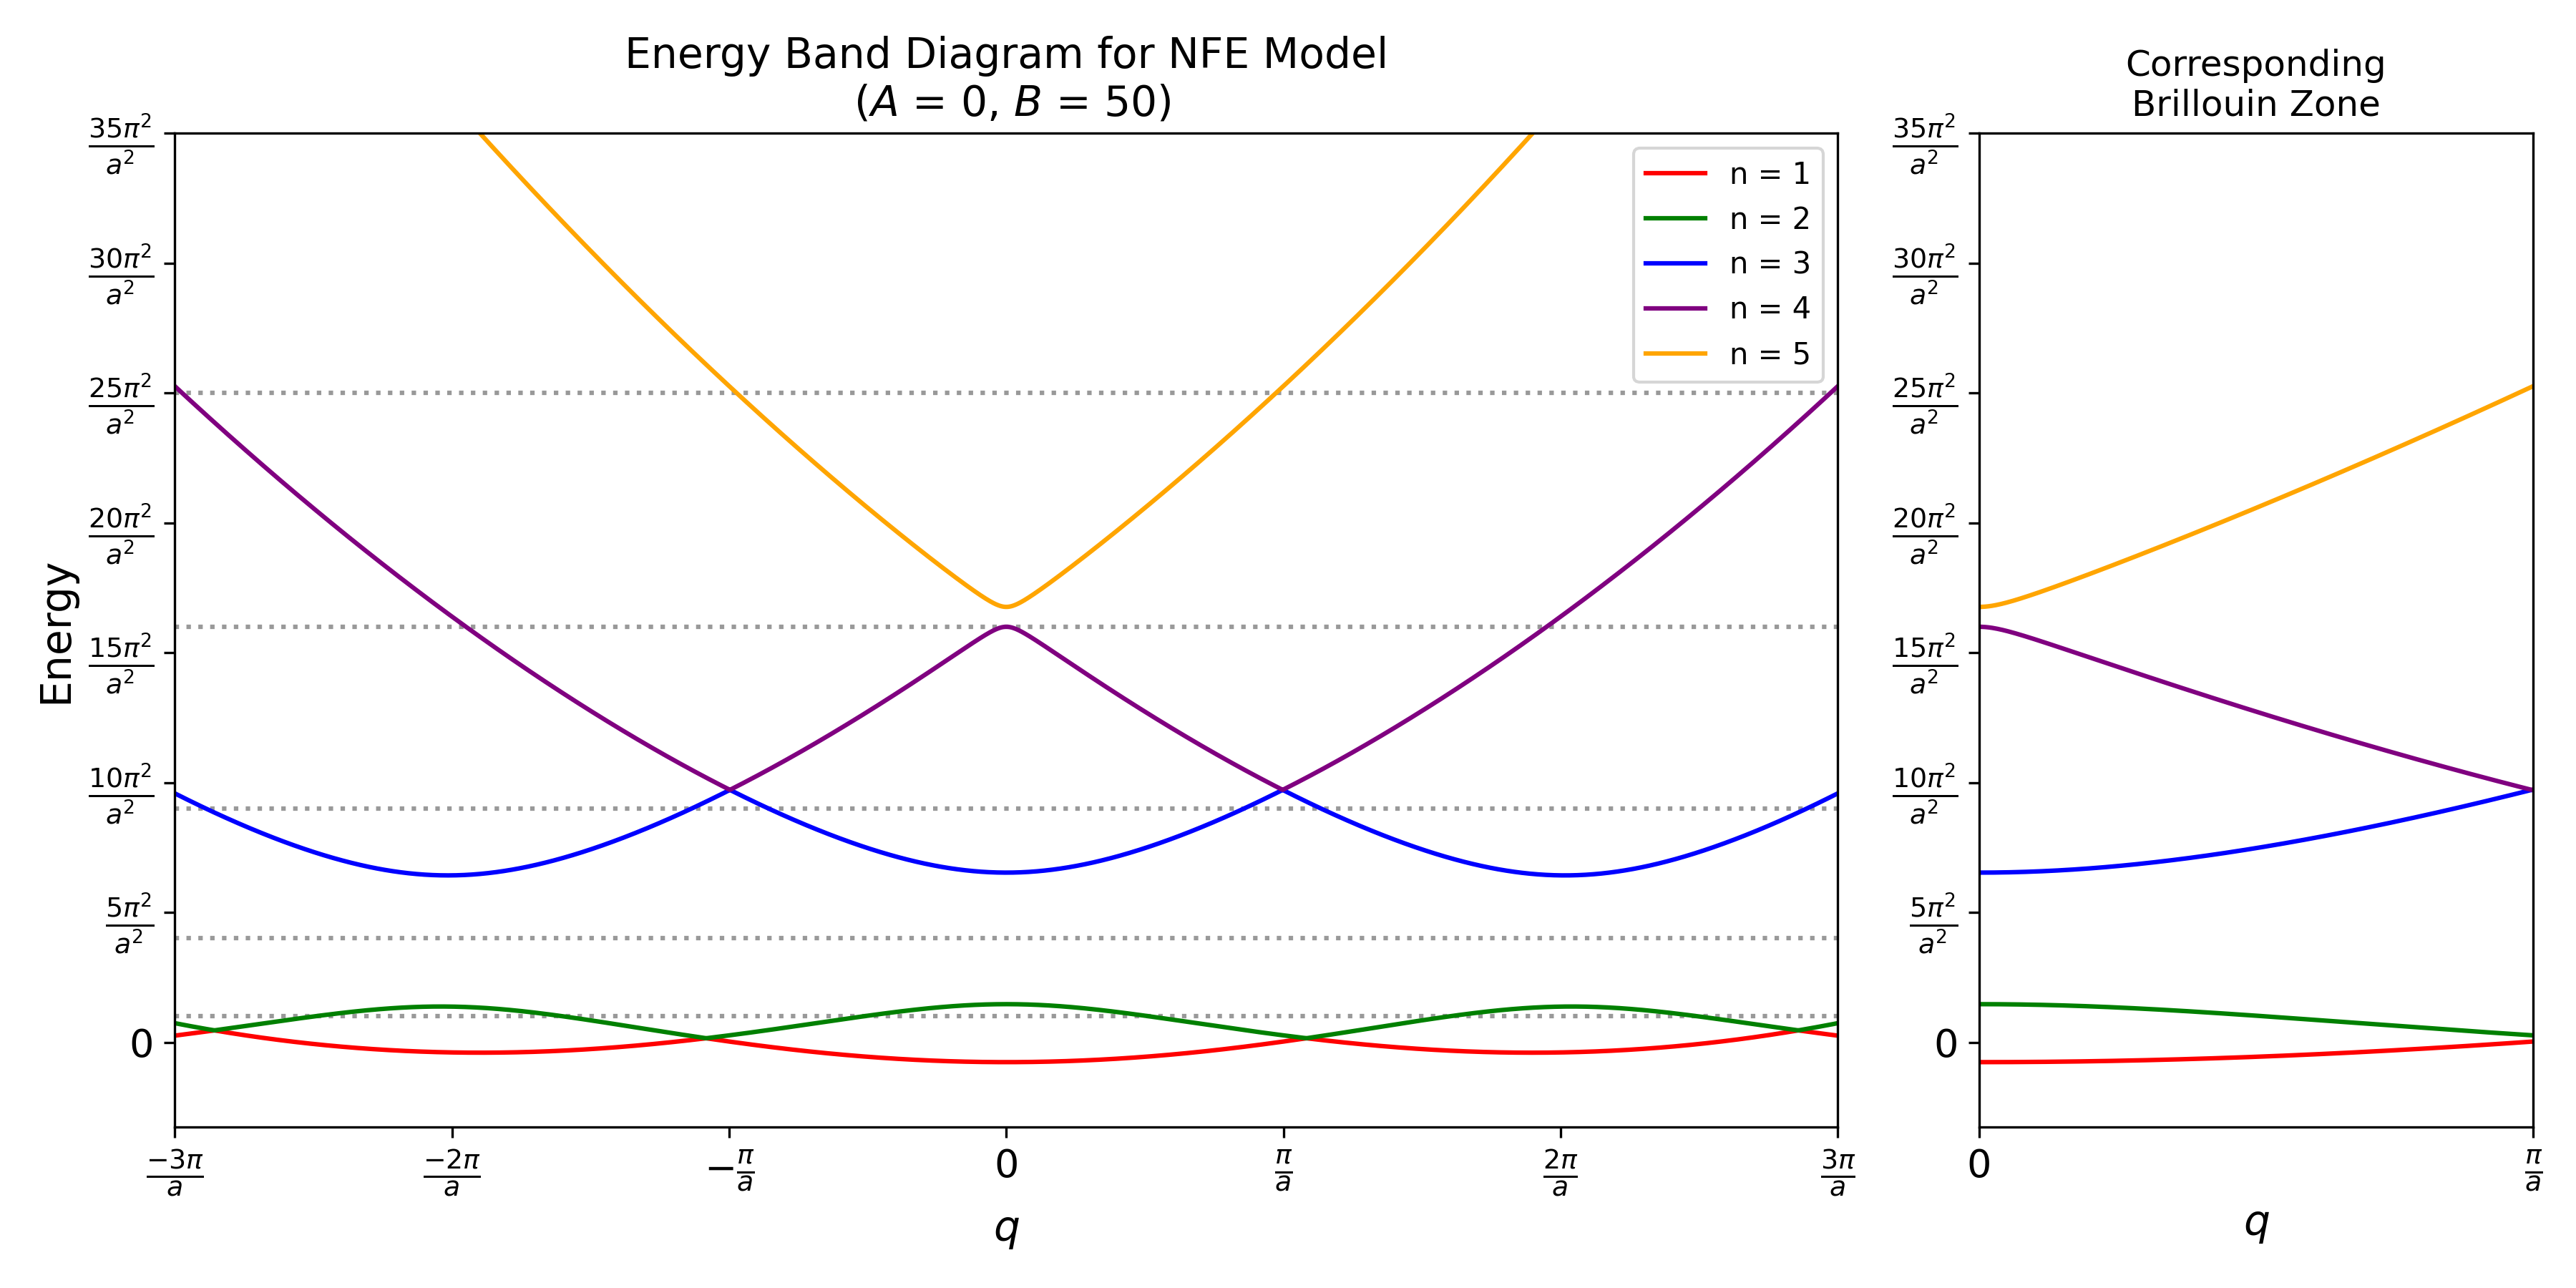
\includegraphics[width=1\linewidth]{images/h2.png}
    \caption{Band Structure for when $A=30$ and $B=0$. As you can see, this opens up a non-zero gap between all the bands at $q=0$ in the Brillouin Zone in decreasing magnitude.}
    \label{h2}
\end{figure}

\subsubsection{Addition of $V_{G_3}$ and $V_{G_4}$}

Now consider a modified potential of the form,

\begin{align*}
    V(x) = A\cos\left(\frac{2\pi x}{a}\right) + B\cos\left(\frac{4\pi x}{a}\right) + C\cos\left(\frac{6\pi x}{a}\right) + D\cos\left(\frac{8\pi x}{a}\right)
\end{align*}

Here, we have introduced a non-zero third and fourth fourier coefficients (with periodicities thrice and four times that $G=1$ respectively). The Hamiltonian matrix has to be modified accordingly by introducing new off-diagonal terms where $m=n\pm 3$ and $m=n\pm 4$.
The resultant band structures are shown below.

The values of the $\Delta E$ in these band gaps can be derived similar to the argument we have provided in Section \ref{1.3}.

\begin{figure}[H]
    \centering
    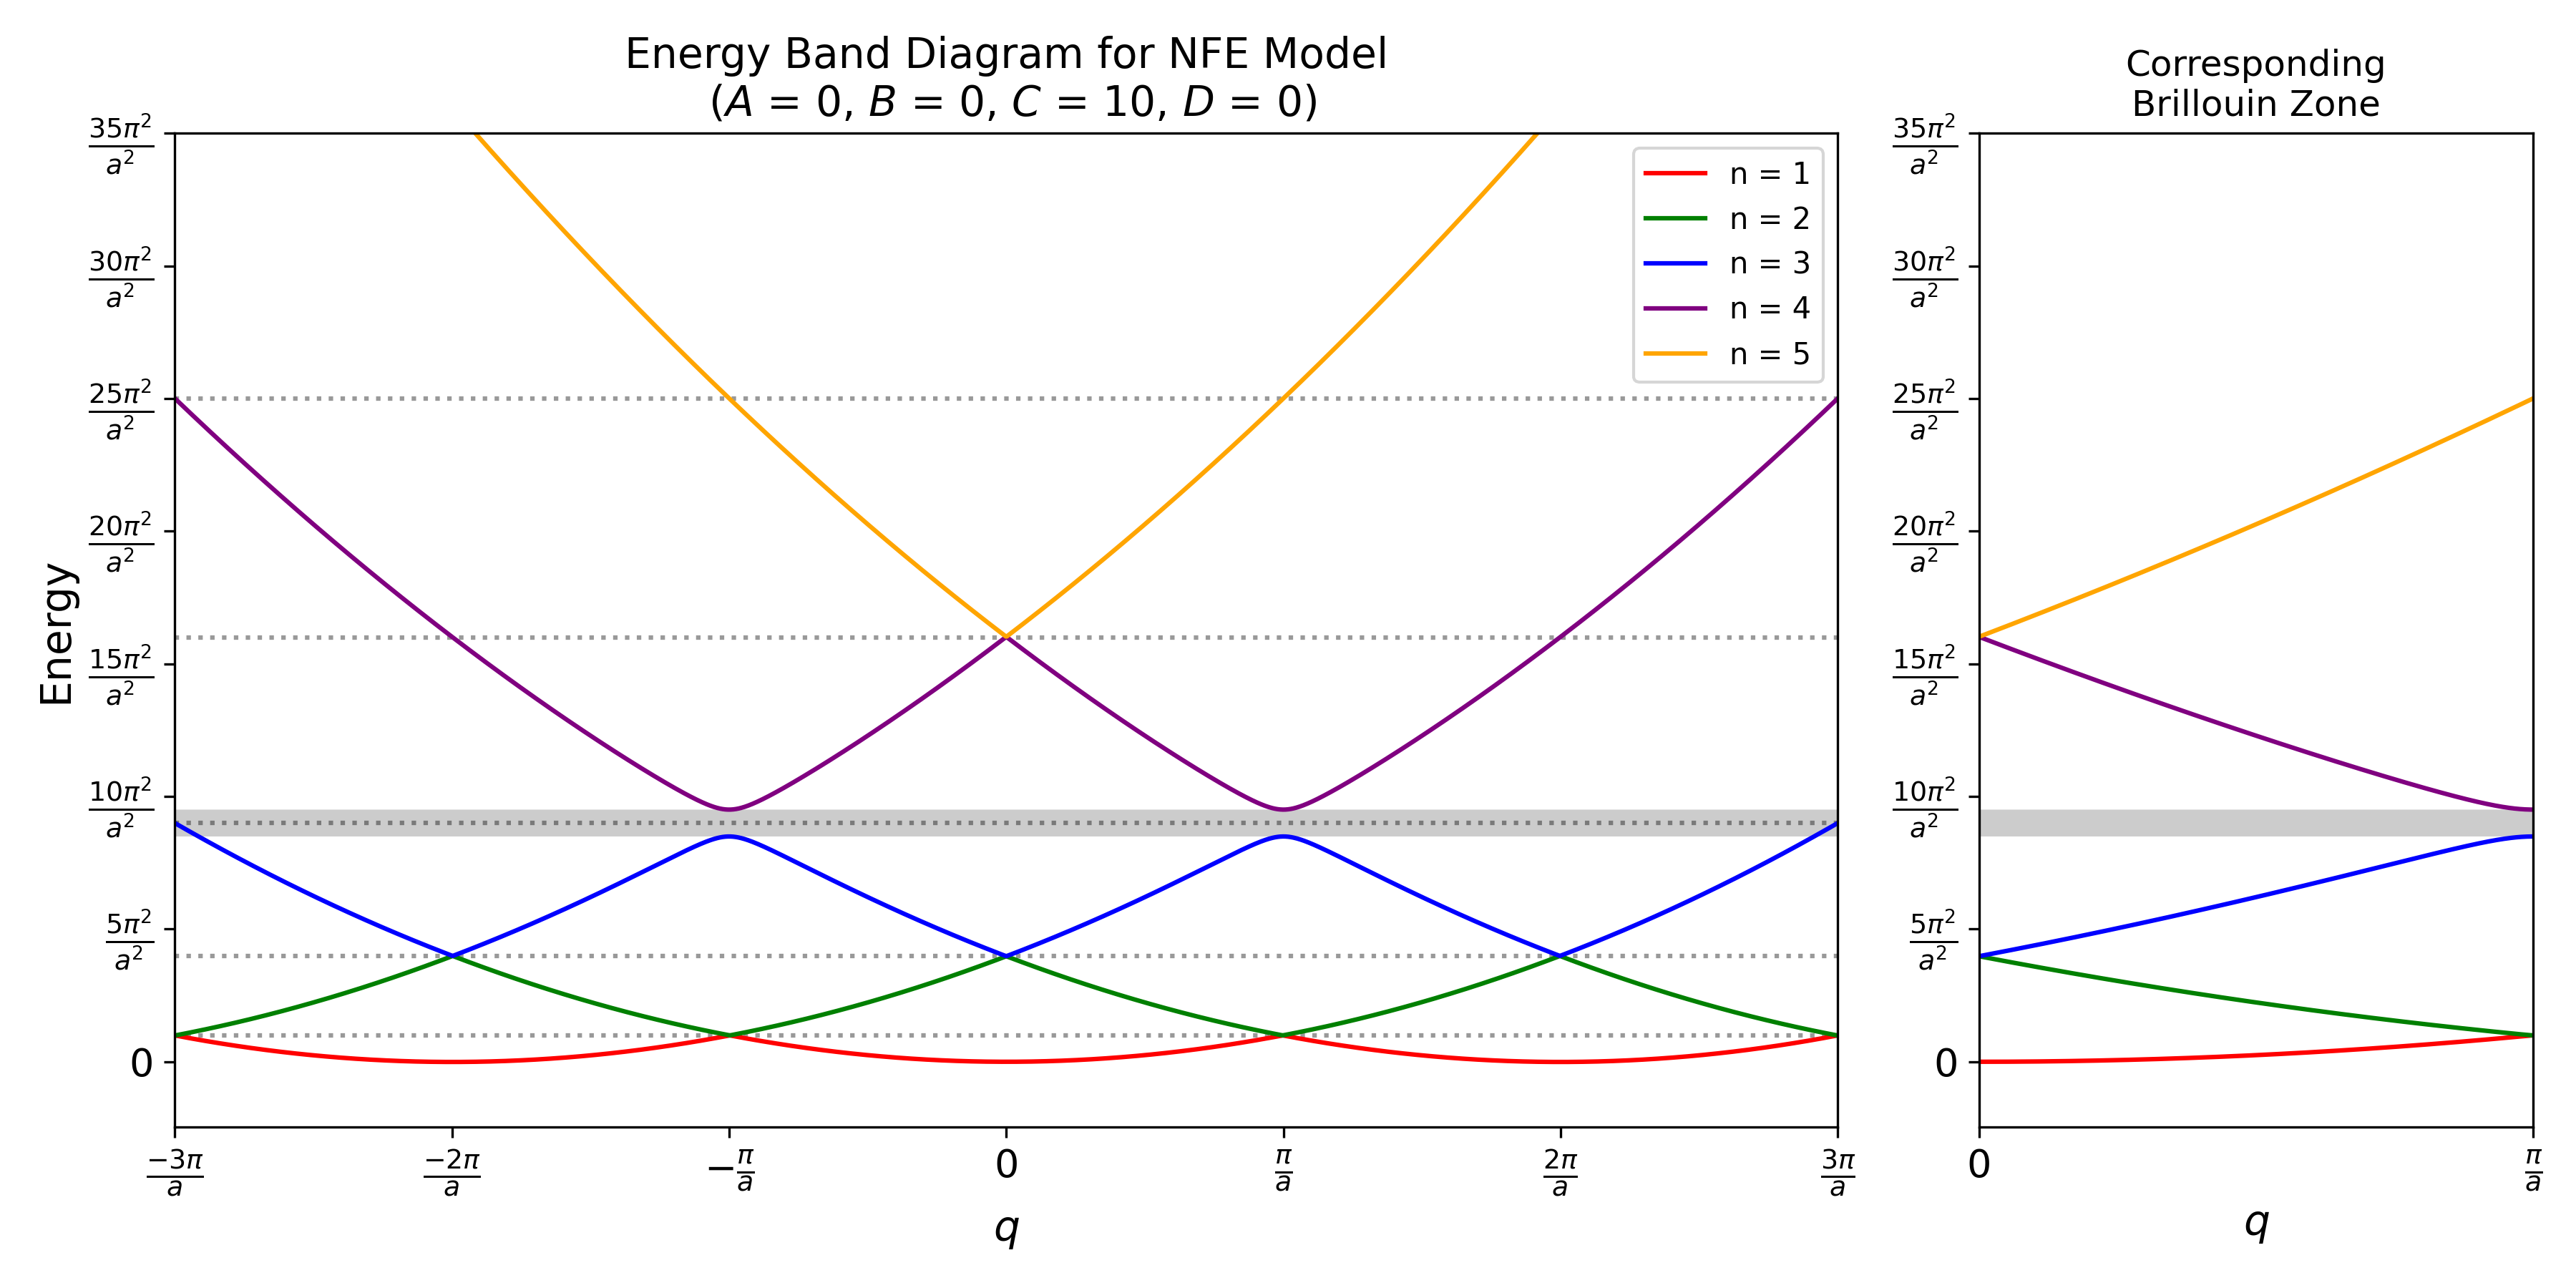
\includegraphics[width=1\linewidth]{images/g3.png}
    \caption{Band Structure for when $A=B=D=0$ and $C=10$. As you can see, this opens up a band gap between the third and the fourth band at $q=\pi/a$ in the Brillouin zone. The magnitude of the bandgap is equal to $C$.}
    \label{g3}
\end{figure}

\begin{figure}[H]
    \centering
    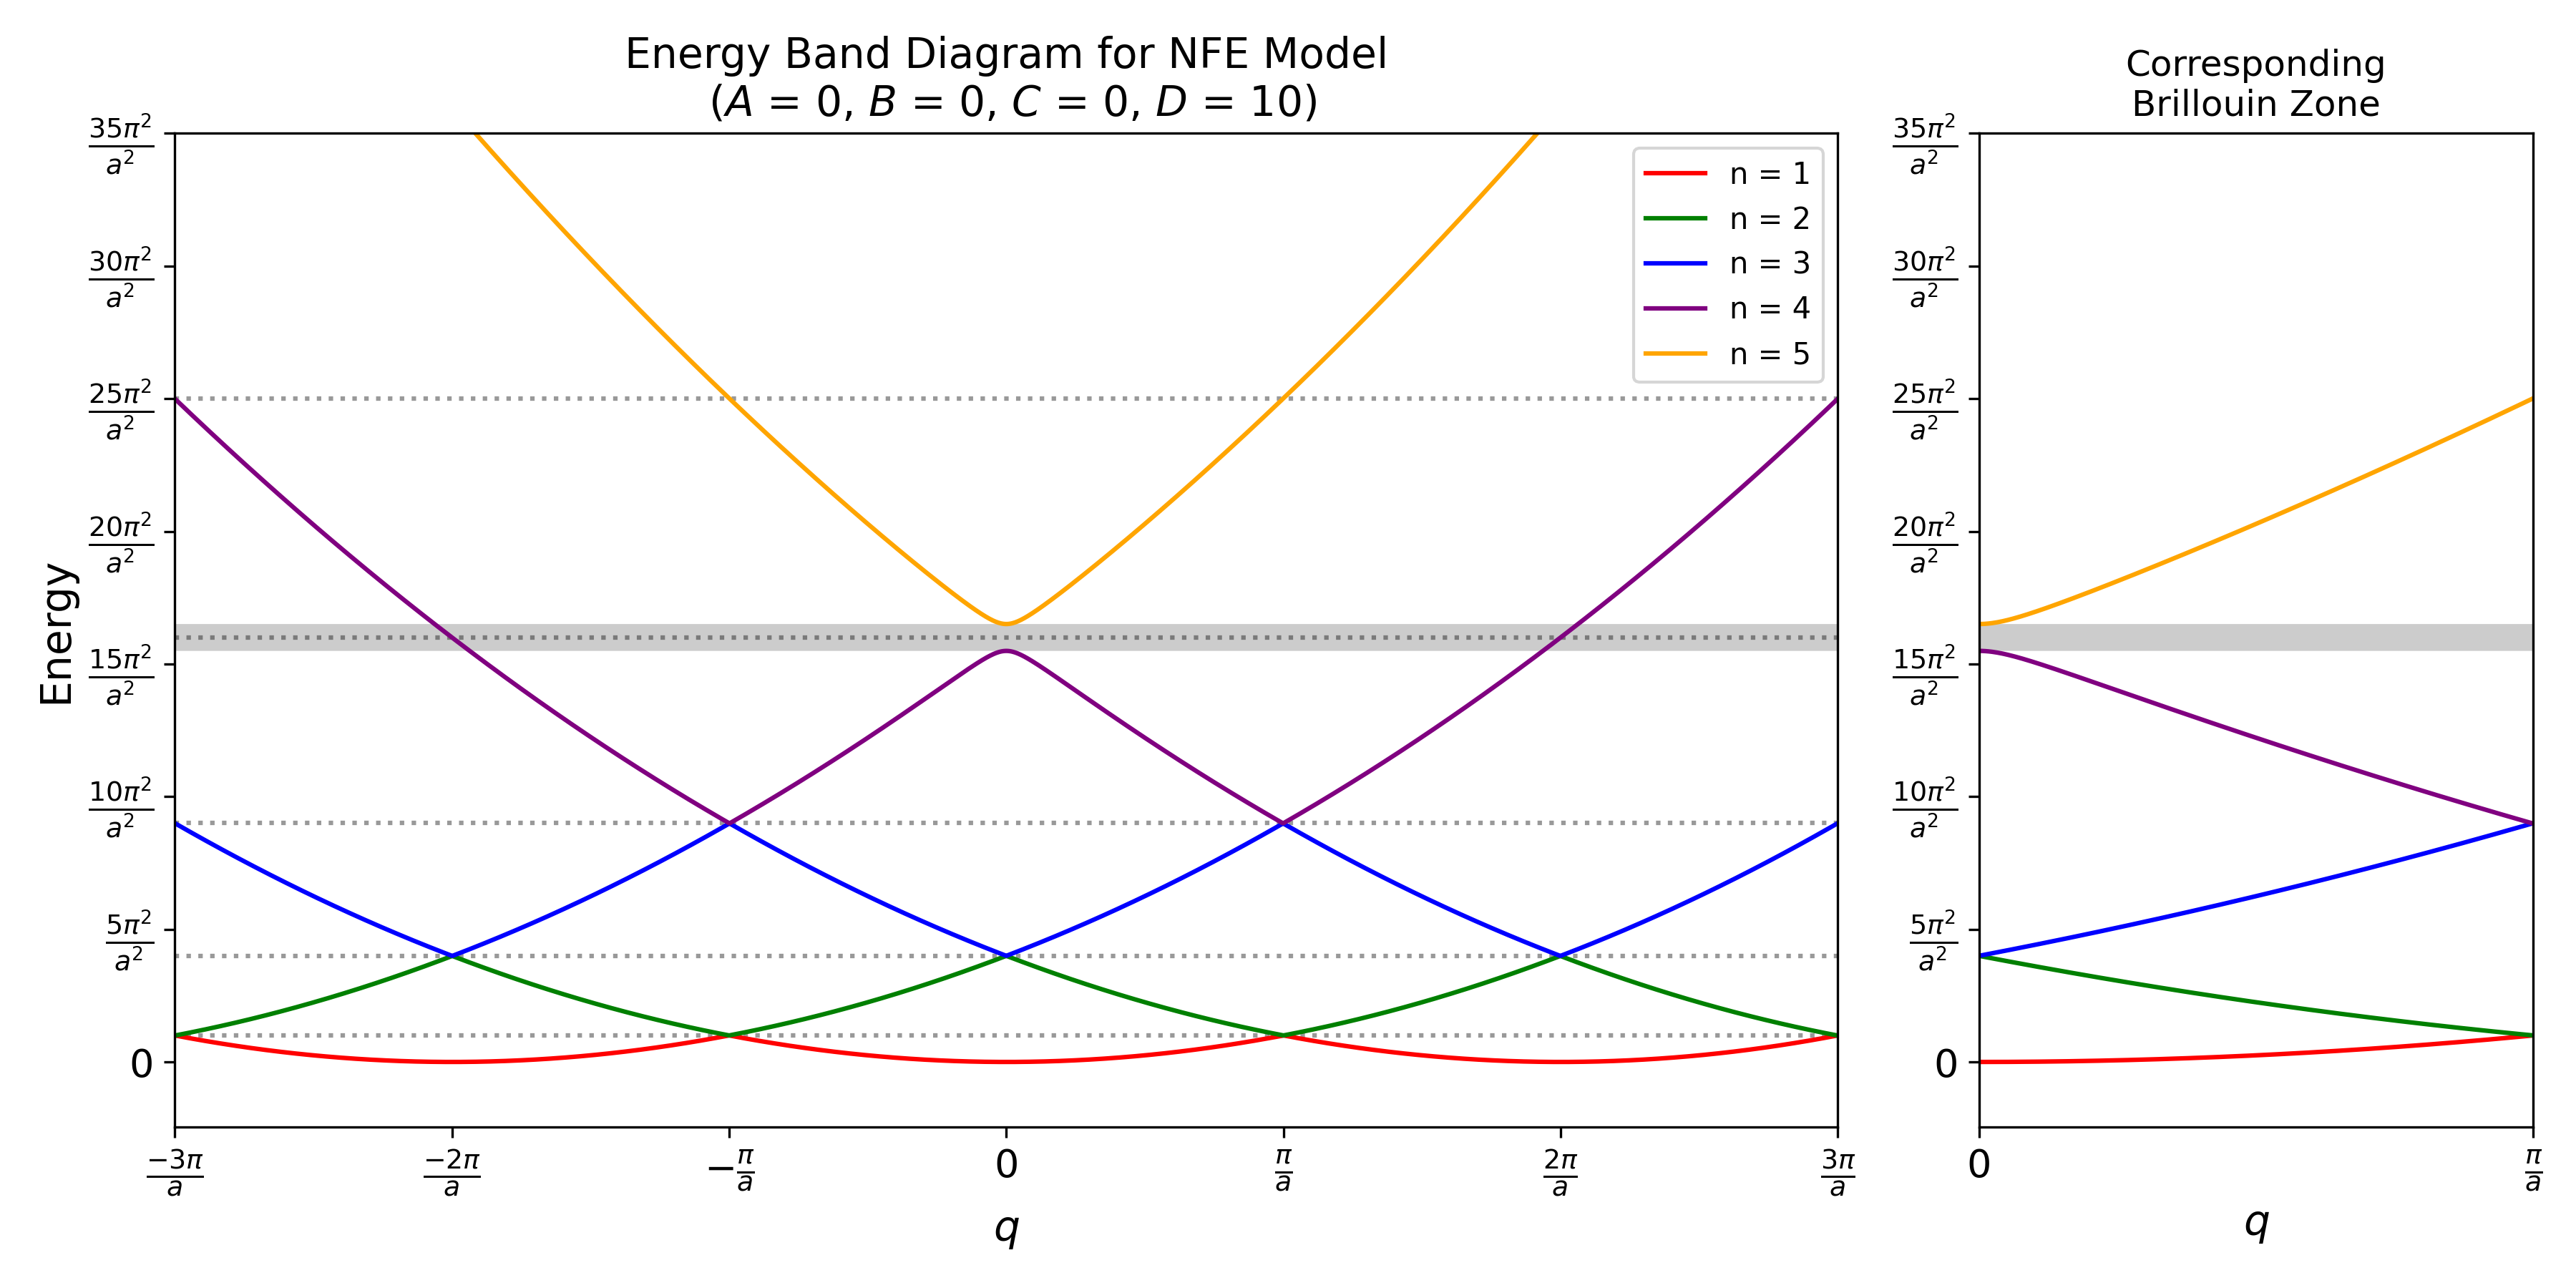
\includegraphics[width=1\linewidth]{images/g4.png}
    \caption{Band Structure for when $A=B=C=0$ and $D=10$. As you can see, this opens up a band gap between the fourth and the fifth band at $q=0$. The magnitude of the bandgap is equal to $D$.}
    \label{g4}
\end{figure}

\section{Discussion \& Conclusion}
Using Python we were able to numerically simulate the band structures of a nearly free electron model, with a potential energy term given by
\begin{align*}
    V(x) &= A\cos\left(\frac{2\pi x}{a}\right) + B\cos\left(\frac{4\pi x}{a}\right)
\end{align*}
To do this, we have diagonalised the appropriate Hamiltonian matrix (construction detailed in Section \ref{1.2}) and have plotted the appropriate eigenvectors corresponding to each energy band.

For small values of potential energy, we have numerically been able to obtain values of bandgap as we estimated in Section \ref{1.3}. The first fourier coefficient ($V_{G_1}$) term leads to a bandgap equal to $|V_{G_1}|$ between the first and second bands. Similarly the second fourier coefficient ($V_{G_2}$) term leads to a bandgap equal to $|V_{G_2}|$ between the second and third bands.

For higher values of $V$ ($>> (\pi/a)^2$), we were able to see that $V_{G_1}$ causes band gaps to open between every pair of bands, in decreasing order of magnitudes. We find that the band corresponding to the first energy state lowers and even goes below 0. Similarly, $V_{G_2}$ causes band gaps to open between every second pair of bands. This is expected as the periodicity of the seond fourier coefficient is twice that of the first one. 

Finally, we also considered the how a non-zero third and fourth order fourier coefficient in the expansion of $V$ will change the band structure of the electron. As expected, we saw that the $V_{G_3}$ opens up a band gap between the third and the fourth bands, of magnitude $|V_{G_3}|$. Similarly, $V_{G_4}$ opens up a band gap between the fourth and the fifth bands, of magnitude $|V_{G_4}|$.

% {\footnotesize
% \section*{References}
% \begin{itemize}
%     \item https://www.eecs70.org/assets/pdf/notes/n8.pdf
%     \item Verbal discussions
% \end{itemize}
% }

\end{document}